%%
%\begin{figure}[htbp]
%\begin{center}
%\includegraphics[width=3cm]{sample.eps}
%\psfig{file=sample.eps,scale=0.6}
%\epsfile{file=sample.eps,scale=0.6}
%\end{center}
%\caption{図の例}
%\label{figure:sample}
%\end{figure}


% このファイルは、筑波大学情報学群情報科学類の
% 卒業研究論文本体のサンプルです。
% このファイルを書き換えて、この例と同じような書式の論文本体を
% LaTeXを使って作成することができます。
% 
% PC環境や、LaTeX環境の設定によっては漢字コードや改行コードを
% 変更する必要があります。
%%
\documentclass[a4paper,11pt]{jreport}

%%【PostScript, JPEG, PNG等の画像の貼り込み】
%% 利用するパッケージを選んでコメントアウトしてください。
\usepackage[dvipdfmx]{graphicx}  
%for includegraphics[width=3cm]{sample.eps}
%\usepackage{epsfig} % for \psfig{file=sample.eps,width=3cm}
%\usepackage{epsf} % for \epsfile{file=sample.eps,scale=0.6}
%\usepackage{epsbox} % for \epsfile{file=sample.eps,scale=0.6}
% MATH
\usepackage{amsmath}
\usepackage{amsfonts}
\usepackage{varioref}
\usepackage[shortlabels]{enumitem}

\newlist{abbrv}{itemize}{1}
\setlist[abbrv,1]{label=,labelwidth=1in,align=parleft,itemsep=0.1\baselineskip,leftmargin=!}


\DeclareMathOperator{\cut}{cut\,}
\DeclareMathOperator{\ii}{I\,}
\DeclareMathOperator{\h}{H\,}
\DeclareMathOperator{\nmi}{NMI\,}
\DeclareMathOperator{\spn}{span\,}
\DeclareMathOperator*{\vol}{vol\,}
\DeclareMathOperator*{\ncut}{Ncut\,}
\DeclareMathOperator*{\argmin}{\arg\!\min}
%\DeclareMathOperator*{\dim}{dim}


%% dvipdfm を使う場合(dvi->pdfを直接生成する場合)
%\usepackage[dvipdfm]{color,graphicx}
%% dvipdfm を使ってPDFの「しおり」を付ける場合
%\usepackage[dvipdfm,bookmarks=true,bookmarksnumbered=true,bookmarkstype=toc]{hyperref}
%% 参考:dvipdfm 日本語版
%% http://hamilcar.phys.kyushu-u.ac.jp/~hirata/dvipdfm/

\usepackage[left=25truemm,top=35truemm,right=25truemm,bottom=50truemm]{geometry}
\usepackage{times} % use Times Font instead of Computer Modern

\setcounter{tocdepth}{3}
\setcounter{page}{-1}

\setlength{\parskip}{0em}
\setlength{\topsep}{0em}

%\newcommand{\zu}[1]{{\gt \bf 図\ref{#1}}}

%% タイトル生成用パッケージ(重要)
\usepackage{coins-jp-utf8}

%% タイトル
%% 【注意】タイトルの最後に\\ を入れるとエラーになります
\title{\underline{Extending the use of the Bethe Hessian} \underline{to Constrained Spectral Clustering}}
%% 著者
\author{Soares Oliveira, Farley}
%% 指導教員
\advisor{櫻井鉄也}

%% 専攻名 と 年月 (提出年月)
%% 年月は必要に応じて書き替えてください。
\heiseiyear{29}  % 平成の年度
\majorfield{ソフトウェアサイエンス主専攻}
%\majorfield{情報システム主専攻}
%\majorfield{知能情報メディア主専攻}
\usepackage[english]{babel}
\renewcommand{\prechaptername}{Chap. }
\renewcommand{\postchaptername}{}




% NORM
\newcommand\norm[1]{\left\lVert#1\right\rVert}


% Integer Intervals
\usepackage{mathtools, stmaryrd}
\usepackage{xparse} \DeclarePairedDelimiterX{\Iintv}[1]{\llbracket}{\rrbracket}{\iintvargs{#1}}
\NewDocumentCommand{\iintvargs}{>{\SplitArgument{1}{,}}m}
{\iintvargsaux#1} %
\NewDocumentCommand{\iintvargsaux}{mm} {#1\mkern1.5mu, \mkern1.5mu#2}

% Algorithms
\usepackage{algorithm}
\usepackage[noend]{algpseudocode}

\makeatletter
\def\BState{\State\hskip-\ALG@thistlm}
\makeatother

% THEOREM NADO

\newtheorem{theorem}{Theorem}[section]
\newtheorem{lemma}[theorem]{Lemma}
\newtheorem{proposition}[theorem]{Proposition}
\newtheorem{conjecture}[theorem]{Conjecture}
\newtheorem{corollary}[theorem]{Corollary}
\newenvironment{proof}[1][Proof]{\begin{trivlist}
\item[\hskip \labelsep {\bfseries #1}]}{\end{trivlist}}
\newenvironment{definition}[1][Definition]{\begin{trivlist}
\item[\hskip \labelsep {\bfseries #1}]}{\end{trivlist}}
\newenvironment{example}[1][Example]{\begin{trivlist}
\item[\hskip \labelsep {\bfseries #1}]}{\end{trivlist}}
\newenvironment{remark}[1][Remark]{\begin{trivlist}
\item[\hskip \labelsep {\bfseries #1}]}{\end{trivlist}}
\newcommand{\qed}{\nobreak \ifvmode \relax \else
      \ifdim\lastskip<1.5em \hskip-\lastskip
      \hskip1.5em plus0em minus0.5em \fi \nobreak
      \vrule height0.75em width0.5em depth0.25em\fi}


\begin{document}
\maketitle
\thispagestyle{empty}
\newpage

\thispagestyle{empty}
\vspace*{20pt plus 1fil}
\parindent=1zw
\noindent
%%
%% 論文の概要(Abstract)
%%
\begin{center}
{\Large \bf Abstract}
\vspace{2cm}
\end{center}
Here you write the abstract of your thesis.

%%%%%
\par
\vspace{0pt plus 1fil}
\newpage

\pagenumbering{roman} % I, II, III, IV 
\tableofcontents
\listoffigures
%\listoftables

\pagebreak \setcounter{page}{1}
\pagenumbering{arabic} % 1,2,3


\chapter{Introduction}
We have two goals in this work.

The first one is to introduce the reader to the spectral theory of clustering and constrained clustering.
We assume the reader is familiar with the basic linear algebra and discrete mathematics which should be common knowledge to any upper division undergraduate student in computer science.
From there, we build up the rudimentary tools of spectral graph theory and show how they can be used to perform clustering and constrained clustering.
All concepts are rigorously defined, and for each proposition we provide either a proof or a direct reference to a proof of it.
Chapters 2 and 4 are mainly comprised of this.

The second goal is to apply the spectral theory introduced to a certain stochastic class of graphs. We explain and define a certain generative graph model known as stochastic block model, describe its main properties, and elucidate which algorithms are effective or not in clustering the graphs generated by it.
After that, we introduce the Bethe Hessian, a special matrix particularly useful for clustering graphs generated by this model.
We then propose an extension of an algorithm for constrained clustering introduced in Chapter 4 which is effective in performing constrained clustering in graphs generated by the stochastic block model.
Chapters 3 and 5 are mainly comprised of this.

Finally, in Chapter 6 we show the results of numerical experiments performed to corroborate the theory presented in this thesis.

\section{Notations}
In this section, we explain some of the mathematical notations used in this thesis that may be unfamiliar to some of the readers.


\begin{abbrv}
\item[$\mathbb N$]: set of non-negative integers.
\item[$\mathbb Z$]: set of integers.
\item[$ \mathbb Z_{>m}$]: set of integers bigger than $m$. Similar for other order relations.
\item[$\mathbb R$]: set of real numbers.
\item[$\mathbb C$]: set of complex numbers 
\item[$\Iintv{m,n}$] $= \{ i \in \mathbb N: m \le i \le n \}$, where $m$ and $n$ are two natural numbers with $m < n$.
\item[$A \times B$] $= \{ (x,y): x \in A \text{ and } y \in B \}$:  Cartesian product of the sets $A$ and $B$.
\item[$A^n$]  $= \{ (x_1, x_2, \cdots, x_n): x_i \in A \text{ for all } i \in \Iintv{1,n} \}$, where $A$ is a set and $n$ is a positive integer: $n$-ary Cartesian power of $A$.
\item[$G = (V,E)$] : the graph $G$ (supposed of order $m$) has $V = \{ v_1, v_2, \cdots, v_m \}$ as its set of vertices and $E$ as its set of edges.
\item[$A_{ij}$] : element corresponding to the $i$-th row and $j$-th column in the matrix $A$.
\item[$\mathbb R ^{m \times n}$] : Set of $m$ by $n$ matrices with real coefficients. Similar for the set $\mathbb C$.
\item[$\mathbb R^n$] $= \mathbb R^{n \times 1}$: set of real column vectors of dimension $n$. To be distinguished from the $n$-ary Cartesian power of $\mathbb R$ from the context. Similar for the set $\mathbb C$.
\item[$\mathbb R^{1 \times n}$]: set of real row vectors of dimension $n$. Similar for the set $\mathbb C$.
\item[$a_{m \times n}$]: $m$ by $n$ matrix where all elements are equal to $a$, where $a \in \mathbb R$.
\item[$ { [a , b]  }  $]  $= \{ x \in \mathbb R: a \le x \le b \} $, where $(a,b) \in \mathbb R^2$.
\item[ ${ ] a , b [ }$ ] $= \{ x \in \mathbb R: a < x < b \}$, where $(a,b) \in \mathbb R^2$. Similar for other combinations.
\item[ $\mathbb P ( \cdot )$]: probability of the event $\cdot$ happening.
\item[$\mathcal N (A)$]: nullspace of the matrix $A$.
\item[$\spn V$]: span of the set of vectors $V$.
\end{abbrv}

Furthermore, $1$ by $1$ complex matrices are considered complex numbers.





\chapter{Spectral clustering}
%%%% The reader may skip this section (...). %%%%
In this chapter we define the clustering problem, describe general ways in which it can be solved, and introduce
spectral clustering as a solution to this problem which uses the Courant-Fischer Min-Max Theorem.
The material here is based mainly on \cite{ng} and \cite{tutorial}.
However, we have changed the notations and some of the presentation, selecting only the relevant parts for the rest of this thesis.
We have also provided several proofs which were omitted in the original papers.\footnote{For example, Proposition~\vref{xtlx}, Proposition~\vref{xtlx2}, Lemma~\vref{cond1}, Lemma~\vref{cond2} and Theorem~\vref{xtxcut}.}
Readers who are already familiar with the derivation of spectral clustering may feel free to skip this chapter. 

\section{The clustering problem}

% How is the clustering problem defined?
Clustering is currently the most popular way of conducting unsupervised learning. 
Given a dataset $\mathcal D$, the objective of clustering is to find a proper partition of $\mathcal D$, $(\mathcal P_1, \mathcal P_2, \cdots, \mathcal P_k)$, where $k \in \mathbb Z_{>1}$ is predetermined by the user of the algorithm, such that the similarity of elements of a same subset $\mathcal P_i$  $(\text{with } i \in \Iintv{1,k})$ are as big as possible and the similarity of elements of different subsets $\mathcal P_i$ and $\mathcal P_j$ $(\text{where } (i,j) \in \Iintv{1,k}^2, i \ne j)$ are as small as possible. 
In other words, a clustering algorithm assigns a label $l \in \Iintv{1,k}$ to each data instance in $\mathcal D$ in such a way that data instances which are similar to each other are assigned the same label.
The way the similarity of elements of a same subset and the similarity of elements of different subsets are calculated depends on the clustering algorithm used. 
We can say the same about the way in which the dataset $\mathcal D$ is represented.

% What are some non-spectral ways of doing clustering?
Clustering may be achieved by several different approaches, each with its own advantages and disadvantages.
Some models and approaches for clustering are:
\begin{itemize}
   \item Strict partioning clustering: each data instance is classified into one cluster based on its similarity with other instances.
      The main approach for this type of clustering is k-means: the algorithm works by iteratively assigning a label to each data instance based on its similarity with each cluster.
      Here, the similarity of a data instance and a cluster is obtained by computing the similarity between the instance and some kind of representative data instance of the cluster, usually some kind of mean vector.
   \item Hierarchical clustering: the data is divided in clusters which make up a hierarchy.
      This type of clustering may be achieved by two main approaches: the agglomerative approach, where each data instance starts in its own cluster, and pairs of clusters are merged as we go up in the hierarchy; and the divisive approach, where all data instances start in a same cluster, and clusters are split as we go down the hierarchy.
      One advantage of hierarchical clustering is that the algorithm user does not need to set the number of subsets $k$ ahead of time.
   \item Overlapping clustering: In the final result, each data instance may be an element of more than one cluster.
      In other words, $(\mathcal P_1, \mathcal P_2, \cdots, \mathcal P_k)$ is not necessarily a partition of $\mathcal D$.
      This approach may be useful when certain data instances naturally pertain to more than one class.
\end{itemize}

% Spectral Clustering? What are the characteristics (advantages) of a spectral approach?
In contrast to the approaches above, spectral clustering works by transforming the data into a graph, constructing a certain matrix associated to this graph called the Laplacian, computing the eigenvalues and eigenvectors of the Laplacian, and finally using this eigeninformation to classify the data.
Although spectral clustering is often more difficult to implement (requiring, e.g., an algorithm to efficiently solve an eigenproblem), it is more general than the more common approaches such as k-means and hierarchial clustering.
This is because spectral clustering may be succesfuly used for data that are arranged in complex shapes (as long as each cluster is connected), since the data is first mapped from their native data space to another one in which connectivity is preserved but geometrical relationships are simplified.

% What are the two forms spectral clustering can be derived?
There are two main approaches with which spectral clustering can be derived.
The first one, the \textit{ideal case} approach, considers regular Laplacian matrices as perturbations of an ideal case in which data points that are to be classified into different clusters are infinitely far apart.
The second one, the \textit{relaxation} approach, considers spectral clustering as a approximation algorithm to solve a original NP-complete discrete optimization problem.
The former is related to the Bethe Hessian spectral lustering algorithm, while the latter is related to the FAST-GE-2.0 algorithm, both of which will be discussed henceforth in this thesis.
For this reason, we will explain both approaches in this chapter.

We show the spectral clustering algorithm below and explain why it outputs a valid result in the subsequent sections.

\begin{algorithm}
\caption{Spectral clustering}\label{spectral_clustering}
\begin{algorithmic}[1]
   \Require 
      \Statex Adjacency Matrix of the graph $G = (V,E)$: $A \in \mathbb R ^ {m \times m}$ 
      \Statex Number of Clusters: $k \in \mathbb Z_{>1}$
   \Ensure 
      \Statex Partition of the set of vertices $V$: $\{ C_1, C_2, \cdots, C_k \} \subseteq V$
      \vspace{0.2 cm}
   \State Compute the normalized Laplacian $L$ of $A$.
   \State Compute the first $k$ eigenvectors $(x_1, x_2, \cdots, x_k) \in (\mathbb R^{m})^k$ of $L$.
   \State Let $X \in \mathbb R^{m \times k}$ be the matrix containing the vectors $x_1, x_2, \cdots, x_k$ as columns.
   \State Form the matrix $Y \in \mathbb R^{m \times k}$ by normalizing the columns of $X$.
   \State Let $(y_1, y_2, \cdots, y_m) \in ( \mathbb R^{1 \times k} )^m$ represent the row-vectors of $Y$.
   \State Cluster $(y_1, y_2, \cdots, y_m)$ using $k$-means into clusters $\{ D_1, D_2, \cdots, D_k \} $.
   \State For each $i \in \Iintv{1,k}$, set $C_i = \{ v_j \in V: y_j \in D_i \}$.
\end{algorithmic}
\end{algorithm}




\section{Preliminary definitions} 
Before entering the discussion of each derivation, we will give some definitions common to both approaches.
Here we will assume that each data instance $d \in \mathcal D$ is a $n$ dimensional column vector, i.e. $\mathcal D \subseteq \mathbb R^{n }$.

\begin{definition}
   Let $\mathcal D$ be a dataset containing $m$ elements. The \textit{similarity matrix} $A \in \mathbb{R}^{m \times m}$ associated with $\mathcal D$ is defined as follows: 
   \begin{equation}
      A_{ij} = s\,(d_i,d_j), \text{ for each } (i,j) \in \Iintv{1,m}^2,
   \end{equation}
   where $s$ is a similarity measure and $d_i \in \mathcal D$ for each $i \in \Iintv{1,m}$.
   In this thesis, we will only consider the \textit{Gaussian similarity measure}, which is given by 
   \begin{equation}
      \begin{split}
         s_G:\,\,\,\,\,\,\,\,   E^2  &\longrightarrow \mathbb R  \\
          (x, y) & \longmapsto \exp \left( -\frac{1}{2 \sigma ^2} {\norm{x - y}}^2 \right),
      \end{split}
   \end{equation}
   where $E$ is a normed vector space with norm $\norm{\cdot}$ and $\sigma \in \mathbb R$ is a parameter set by the user which controls the width of the neighborhoods.
\end{definition}

We can think of the similarity matrix above as encoding the \textit{adjacency matrix} of a weighted graph $G_{\mathcal D} = (V_{\mathcal D}, E_{\mathcal D})$ representing the dataset $\mathcal D$. 
In this case, each element $A_{ij}$ of $A$ represents the weight of an edge connecting the vertices $(v_i, v_j) \in {V_{\mathcal D}}^2$.

\begin{remark}
It is convenient here to establish a bijective relationship between the similarity matrix of a dataset and the adjacency matrix of graph.
   In other words, although we have seen that we may obtain a new graph (represented by an adjacency matrix $A$) from a dataset with similarity matrix $A$, we may also obtain a new dataset (represented by a similarity matrix $A$) from a graph with adjacency matrix $A$.
\end{remark}

\begin{definition}
   Let $A \in \mathbb R ^{m \times m}$ be the adjacency matrix of a graph $G = (V, E)$. The \textit{unnormalized Laplacian matrix} of the graph $G$ is defined by
   \begin{equation}
      L_0 = D - A,
   \end{equation}
   where $D \in \mathbb R ^{m \times m}$ is defined to be the diagonal matrix whose $D_{ii}$ elements are given by the sum of the elements of the matrix $A$'s $i$-th row, for all $i \in \Iintv{1,m}$.
\end{definition}

\begin{definition}\label{unnormalized}
   Let $L_0 \in \mathbb R ^{m \times m}$ be the unnormalized Laplacian matrix of a graph $G = (V, E)$. The \textit{normalized Laplacian matrix} of the graph $G$ is defined by
   \begin{equation}
      L = D^{-1/2}L_0D^{-1/2},
   \end{equation}
   where $D \in \mathbb R ^{m \times m}$ is defined to be the diagonal matrix whose $D_{ii}$ elements are given by the sum of the elements of the matrix $A$'s $i$-th row, for all $i \in \Iintv{1,m}$. 
\end{definition}

\section{Ideal case approach}
Here we will consider the ideal case for spectral clustering where, for all $(i,j) \in \Iintv{1,m}^2$, $A_{ij} = 0$ whenever $d_i$ and $d_j$ are in different clusters, and $A_{ij} > 0$ otherwise.
We will only consider the case where the number of clusters $k$ is $3$ and we will assume that, for all $(i,j) \in \Iintv{1,m}^2$, $d_i \in \mathcal D$ are ordered in such a way that $i < j$ whenever the label of $d_i$ is smaller than the label of $d_j$ (remember that the labels $l$ are elements of $\Iintv{1,k}$).
The argument, however, can be easily extended to a general case.

In this section, for algebraic convenience, we will use an alternative definition for the unnormalized Laplacian matrix: $L_{\text{new}} = D^{-1/2}AD^{-1/2}$, instead of $L = D^{-1/2}L_0D^{-1/2}$.
The use of this trick is justified by the fact that, since $L_0 = D - A$, we have that $L_{\text{new}} + L = I_m$, where $I_m$ is the identity matrix of order $m$.
Therefore $L_{\text{new}}$ and $L$ possess the same eigenvectors, and, for each $i \in \Iintv{1,m}$, if $\lambda _i$ is an eigenvalue of $L$, then $1 - \lambda _i$ is an eigenvalue of $L_{\text{new}}$. 
Outside of this section, however, we will use the normal definition of unnormalized Laplacian as given in the previous section.

Before entering the derivation, we need to outline a result.

\begin{proposition}
   \label{bigeigenvalue}
   Let $G$ be a connected graph of order $m$.
   The normalized Laplacian associated with $G$ has the eigenvalue $1$ with positive eigenvector.
   Furthermore, all the other eigenvalues are smaller than $1$.
\end{proposition}

This is a basic result in spectral graph theory.
A proof may be found in, e.g., \cite{mahoney}.

Consider the dataset $\mathcal D$ corresponding to the graph $G$ and let $d_i \in \mathcal D$ for all $i \in \Iintv{1,m}$. Since $A_{ij} = 0$ whenever $d_i$ and $d_j$ are in different clusters, $A \in \mathbb{R} ^{m \times m}$ may be expressed as a block matrix as follows:

\begin{equation}
   A = 
   \begin{bmatrix}
      A^{(1)} & 0_{m_1 \times m_2} & 0_{m_1 \times m_3} \\
      0_{m_2 \times m_1} & A^{(2)} & 0_{m_2 \times m_3} \\
      0_{m_3 \times m_1} & 0_{m_3 \times m_2} & A^{(3)}
   \end{bmatrix}.
\end{equation}

Here, all the elements of the three matrices $A^{(1)} \in \mathbb R^{m_1 \times m_1}$, $A^{(2)} \in \mathbb R^{m_2 \times m_2}$ and $A^{(3)} \in \mathbb R ^{m_3 \times m_3}$ are positive (that is, all their elements are positive) and we have that $m_1+m_2+m_3 = m$. 
From now on in this section, to avoid verbosity, we will omit the subscripts of the $0$ matrices.

It follows from the definitions that the normalized Laplacian $L$ and the diagonal matrix $D$ can be expressed as block matrices in a similar way:

\begin{equation}
 D =
   \begin{bmatrix}
      D^{(1)} & 0 & 0 \\
      0 & D^{(2)} & 0 \\
      0 & 0 & D^{(3)}
   \end{bmatrix}
   \,\,\,\,\,\text{ and }\,\,\,\,\,
   L = 
   \begin{bmatrix}
      L^{(1)} & 0 & 0 \\
      0 & L^{(2)} & 0 \\
      0 & 0 & L^{(3)}
   \end{bmatrix},
\end{equation}

where $D^{(1)} \in \mathbb R ^{m_1 \times m_1}$, $D^{(2)} \in \mathbb R ^{m_2 \times m_2}$ and $D^{(3)} \in \mathbb R ^{m_3 \times m_3}$ are themselves diagonal matrices and $L^{(1)} \in \mathbb R ^{m_1 \times m_1}$, $L^{(2)} \in \mathbb R ^{m_2 \times m_2}$ and $L^{(3)} \in \mathbb R ^{m_3 \times m_3}$ are positive normalized Laplacians of each element of the partition $(\mathcal P_1, \mathcal P_2, \mathcal P_3)$.
Here, the following relation holds for each $i \in \{1, 2, 3 \}$:

\begin{equation}
   L^{(i)} = \left( D^{(i)} \right) ^{-1/2} A^{(i)} \left( D^{(i)} \right) ^{-1/2}.
\end{equation}

Since the matrix $L$ is block-diagonal, its set of eigenvalues $\sigma _L$ is given by the union of the set of eigenvalues of each block $L_1$, $L_2$ and $L_3$, respectively $\sigma_{L_1}$, $\sigma_{L_2}$ and $\sigma_{L_3}$.
Furthermore its eigenvectors are the same as the ones of $L_1$, $L_2$ and $L_3$, provided that they are ``extended'' with $0$ elements as necessary. 
The proof of this claim may also be found in \cite{mahoney}.

By Proposition~\vref{bigeigenvalue}, we know that each $L^{(i)}$ ($i \in \{1, 2, 3 \}$) has $1$ as an eigenvalue with positive eigenvector, which we denote by $x_1^{(i)} \in {\mathbb R_{>0}}^{m_i} $. Furthermore, all other eigenvalues of each $L^{(i)}$ are smaller than $1$.
This implies that $L$ has $1$ as an eigenvalue with multiplicity $3$.
Let $X$ be the matrix containing the eigenvectors associated with these eigenvalues as columns. We have that 

\begin{equation}
   X =
   \begin{bmatrix}
      x_1^{(1)} & 0 & 0 \\
      0 & x_1^{(2)} & 0 \\
      0 & 0 & x_1^{(3)}
   \end{bmatrix}
   \in \mathbb R^{m \times 3}.
\end{equation}

However, from elementary linear algebra, we know that for a Hermitian matrix if $v_1$ and $v_2$ are two eigenvectors associated with a certain eigenvalue, so is $\alpha v_1 + \beta v_2$, for all $(\alpha, \beta) \in \mathbb R ^2$.
Since the normalized Laplacian is Hermitian, we could have picked any other three eigenvectors spanning the same subspace as the ones above.
The actual eigenvectors we obtain may depend on the small perturbations in the normalized Laplacian and the eigensolver used.
This means that we could have gotten $XR$ instead of $X$, for any orthogonal matrix $R \in \mathbb{R}^{3 \times 3}$.
Therefore, we make the transformation $X \longmapsto XR$ to the matrix above in our analysis.

By normalizing the rows of the matrix $X$, we construct the matrix $Y \in \mathbb{R}^{m \times 3}$ as follows:

\begin{equation}\label{y}
   Y = 
   \begin{bmatrix}
      1_{m_1 \times 1} & 0 & 0 \\
      0 & 1_{m_2 \times 1} & 0 \\
      0 & 0 & 1_{m_3 \times 1} 
   \end{bmatrix}R.
\end{equation}

If we let ${R_1}^T \in \mathbb{R}^{1 \times 3}$, ${R_2}^T \in \mathbb{R}^{1 \times 3}$ and ${R_3}^T \in \mathbb{R}^{1 \times 3}$ represent the rows of the matrix $R$, Equation~\vref{y} tells us that the $i$-th row of $Y$ is given by ${R_j} ^T$, where $i \in \Iintv{1,m}$, $j \in \{1, 2, 3 \}$ and $d_i \in \mathcal P_j$ (i.e. the label of the $i$-th data instance is $j$).

As a result, the rows of the matrix $Y$ related to the same label $i$ will cluster in the same point ${R_i}^T$.
Furthermore, from the fact that $R$ is an orthogonal matrix, we deduce that rows of $Y$ corresponding to different labels will cluster in points (located in the unit sphere) that are perpendicular to each other. 
This permits us to use the rows of the matrix $Y$ to easily recover the labels of each $d_i \in \mathcal D$, with $i \in \Iintv{1,m}$, by e.g. applying the k-means algorithm to these rows.

Needless to say, most matrices we deal with are not in the ideal form we assumed they were in this section's discussion.
However, we can think of a general matrix $A$ as being of the norm $A = A_{\text{ideal}} + E$, where $A_{\text{ideal}}$ is a matrix in the ideal form we discussed in this section and $E$ represents the perturbation from the ideal case.
As long as the norm of $E$ is small enough, it is possible to prove that a spectral algorithm based on the approach of this section works.
A more detailed description of the approach used in this section can be found in \cite{ng}.


\section{Relaxation approach}
In this section we will derive the same spectral clustering algorithm as we did in the last section by framing the clustering problem as a discrete optimization problem and relaxing it so it is not discrete anymore.
Before doing that, however, we need to give some definitions and outline some preliminary results.

\subsection{Background}

% Define Cut and NCut
\begin{definition}
   Let $G = (V,E)$ be a graph of order $m$ with adjacency matrix $A \in \mathbb R^{m \times m}$, and let $C$ be a proper subset of the set of vertices $V$. 
   Set $\overline{C} = V \setminus C$.
   The \textit{cut} of the subset $C$ is defined as follows:
   \begin{equation}
      \cut (C) = \sum_{\substack{v_i \in C \\ v_j \notin \overline C }} A_{ij}.
   \end{equation}
   When multiple graphs are under discussion, there are cases in which we write the name of the graph considered as in $\cut _G \,(C)$ to make things clearer.
\end{definition}

The cut of a set of vertices $C$ is a measure of how much the elements of $C$ are connected with the vertices of $\overline C$.
For that reason, it is minimized when $C$ is a separated component. 
One may try, then, to conduct clustering by minimizing the cut of the several elements of a proper partition of $V$.
However, a problem with this idea is that an eventual algorithm trying to achieve this objective might minimize the cut by separating individual vertices from the rest of the graph, which is not what we desire.
A possible approach to deal with this complication is to normalize the cut in such a way that small clusters are ``penalized''.
This leads to the next definition.

\begin{definition}
   Let $G = (V,E)$ be a graph of order $m$ with adjacency matrix $A \in \mathbb R^{m \times m}$, and let $(C_1, C_2, \cdots, C_k)$, where $k \in \Iintv{2,m}$, be a proper partition of the set of vertices $V$.
   The \textit{normalized cut} of the partition $(C_1, C_2, \cdots, C_k)$ is defined as the following quantity:
   \begin{equation}
      \ncut (C_1, C_2, \cdots, C_k) = \sum _{i = 1}^k \frac{\cut (C_i)}{\vol(C_i)}.
   \end{equation}
   Here, $\vol (C_i)$ denotes the sum of the degrees of all the vertices $v \in C_i$ for each $i \in \Iintv{1,k}$.
\end{definition}

With this definition, we can think of the objective of spectral clustering as follows: given a graph $G=(V,E)$, and the number of clusters $k$, we wish to find a proper partition $(C_1, C_2, \cdots, C_k)$ of $V$ such that $\ncut (C_1, C_2, \cdots, C_k)$ is minimized. Unfortunately, this discrete optimization problem cannot be solved efficiently by brute force (more on this later). Therefore we will show how to derive a way of minimizing this quantity for $k = 2$ by relaxation. For the general case, the reader may consult \cite{tutorial}.

In the following proposition, we will show a useful form for expressions of the type $x^TLx$, where $L$ is a Laplacian matrix and $x$ is a real vector.
As we will see later, this will come handy when we want to find relationships between Laplacian matrices and the normalized cut of certain partitions.

\begin{proposition}\label{xtlx}
   Let $G = (V,E)$ be a graph of order $m$ with adjacency matrix $A \in \mathbb R^{m \times m}$, and let $L_0$ be the unnormalized Laplacian matrix associated with $G$. Let $x \in \mathbb R^{m }$ be a real vector. Furthermore, for each $i \in \Iintv{1,m}$, let $d_i$ denote the degree of the vertex $v_i$. Then we have
   \begin{equation}
      x^TL_0x = \frac{1}{2}\sum_{i,j = 1}^m A_{ij} \left( x_i - x_j \right)^2.
   \end{equation}
\end{proposition}

\begin{proof}
   \begin{equation*} 
      \begin{split}
         x^TL_0x &= x^TDx - x^TAx \\
         &= \sum_{i=1}^m d_i{x_i}^2 - \sum_{i,j = 1}^m x_i  x_j A_{ij}  \\
         &= \frac{1}{2} 2 \sum_{i=1}^m \left( \sum_{j=1}^mA_{ij} \right){x_i}^2 - \frac{1}{2}\sum_{i,j = 1}^m 2x_i  x_j A_{ij}  \\
         &= \frac{1}{2} \sum_{i,j=1}^m (x_i^2 +x_j^2 - 2x_ix_j)A_{ij} \\
         &= \frac{1}{2} \sum_{i,j=1}^m A_{ij} \left( x_i - x_j \right) ^2
      \end{split}
   \end{equation*} \qed
\end{proof}

The proposition above allows us to say the following:

\begin{corollary}\label{unnormalizedLaplacianProperties}
   The unnormalized Laplacian $L_0$ of a graph $G$ has the following properties:
   \begin{enumerate}
      \item It is positive semidefinite.
      \item The vector $1_{m \times 1}$ is one of its eigenvectors with corresponding eigenvalue $0$.
      \item Thus its eigenvalues can be written as $\lambda_1 \ge \lambda_2 \ge \cdots \ge \lambda_m = 0$.
   \end{enumerate}
\end{corollary}

And here we prove the generalization of the result above.

\begin{proposition}\label{xtlx2}
   Let $G = (V,E)$ be a graph of order $m$ with no isolated vertices and with similarity matrix $A \in \mathbb R^{m \times m}$, let $L$ be the normalized Laplacian matrix associated with $G$, and let $x \in \mathbb R^{m} $ be a real vector. Furthermore, for each $i \in \Iintv{1,m}$, let $d_i$ denote the degree of the vertex $v_i$. Then we have
   \begin{equation}
      x^TLx = \frac{1}{2}\sum_{i,j = 1}^m A_{ij} \left( \frac{x_i}{\sqrt{d_i}} - \frac{x_j}{\sqrt{d_j}} \right)^2.
   \end{equation}
\end{proposition}

\begin{proof}
   \begin{equation*} 
      \begin{split}
         x^TLx &= x^T D ^{-1/2} L_0 D^{-1/2} x \\
         &= x^Tx - x^TD^{-1/2}AD^{-1/2}x \\
         &= \sum_{i=1}^m {x_i}^2 - \sum_{i,j = 1}^m x_i  x_j \frac{A_{ij}}{\sqrt{d_i d_j}}  \\
         &= \frac{1}{2} \left( \sum_{i=1}^m {x_i}^2 - 2\sum_{i,j = 1}^m \frac{x_i}{\sqrt{d_i}} \frac{x_j}{\sqrt{d_j}} A_{ij} + \sum_{j=1}^m {x_j}^2 \right) \\
         &= \frac{1}{2} \left( \sum_{i=1}^m \left( \frac{x_i}{\sqrt{d_i}} \right) ^2 d_i - 2\sum_{i,j = 1}^m \frac{x_i}{\sqrt{d_i}} \frac{x_j}{\sqrt{d_j}} A_{ij} +  \sum_{j=1}^m \left( \frac{x_j}{\sqrt{d_j}} \right) ^2 d_j \right) \\
         &= \frac{1}{2} \left( \sum_{i=1}^m \left( \frac{x_i}{\sqrt{d_i}} \right) ^2 \left( \sum_{j=1}^m A_{ij} \right) - 2\sum_{i,j = 1}^m \frac{x_i}{\sqrt{d_i}} \frac{x_j}{\sqrt{d_j}} A_{ij} +  \sum_{j=1}^m \left( \frac{x_j}{\sqrt{d_j}} \right) ^2 \left( \sum_{i=1}^m A_{ij} \right) \right) \\
         &= \frac{1}{2} \sum_{i,j=1}^m \left( \left( \frac{x_i}{\sqrt{d_i}} \right)^2 - 2\frac{x_i}{\sqrt{d_i}}\frac{x_j}{\sqrt{d_j}} + \left( \frac{x_j}{\sqrt{d_j}} \right) ^2 \right) A_{ij} \\
         &= \frac{1}{2} \sum_{i,j=1}^m A_{ij} \left( \frac{x_i}{\sqrt{d_i}}- \frac{x_j}{\sqrt{d_j}} \right)^2. \qed
      \end{split}
   \end{equation*}\qed
\end{proof}

The proposition above allows us to say the following:

\begin{corollary}
   The normalized Laplacian $L$ of a graph $G$ has the following properties:
   \begin{enumerate}
      \item It is positive semidefinite.
      \item The vector $D^{1/2} \, 1_{m \times 1}$ is one of its eigenvectors with corresponding eigenvalue $0$.
      \item Thus its eigenvalues can be written as $\lambda_1 \ge \lambda_2 \ge \cdots \ge \lambda_m = 0$.
   \end{enumerate}
\end{corollary}

Finally, before entering the second derivation of spectral clustering proper, we need to state two theorems which relate optimization of expressions of the form $x^TMx$ and eigenvalues.
These theorems are collectively known as \textit{Courant-Fischer Min-Max Theorems}.
   It is worthy to note here that the Propositions~\ref{xtlx}~and~\vref{xtlx2} are also important because, as we will see next, the generalized Courant-Fischer Min-Max Theorem requires that one of the matrices concerned be positive semidefinite. 

\begin{theorem} \label{minmax1}
   Let $m$ denote a positive integer, let $M \in \mathbb{C}^{m \times m}$ be a Hermitian matrix and denote its eigenvalues by $\lambda_1 \ge \lambda_2 \ge \cdots \ge \lambda_m$. 
   Assume $U$ and $V$ denote linear subspaces of $\mathbb C^{m }$.
   Then for all $i \in \Iintv{1,m}$ the following holds:
\begin{equation}
   \lambda_i = \min_{\dim (U) = i} \max_{\substack{x \in U \\ x \ne 0_{m \times 1}}} \frac{x^HMx}{x^Hx} = \max_{\dim (V) = m-i+1} \min_{\substack{x \in V \\ x \ne 0_{m \times 1}}} \frac{x^HMx}{x^Hx}.
\end{equation}
\end{theorem}

\begin{theorem} \label{minmax2}
   Let $m$ denote a positive integer, let $M \in \mathbb {C} ^{m \times m}$ be a Hermitian matrix and $N \in \mathbb C ^{m \times m}$ be a Hermitian positive semidefinite matrix such that $\mathcal N (N)  \subseteq \mathcal N (M)$.
   Assume $U$ and $V$ denote linear subspaces of $\mathbb C^{m }$.
   Denote by $r$ the rank of matrix $M$ and by $\lambda_1 \ge \lambda_2 \ge \cdots \ge \lambda_r$ the generalized eigenvalues of the pencil $(M,N)$.
   Then for all $i \in \Iintv{1,r}$ the following holds:
   \begin{equation}
      \lambda_i = \min_{\substack{ \dim U = i \\ U \bot \mathcal N (N)}} \max_{x \in U} \frac{x^HMx}{x^HNx} = \max_{\substack{\dim  V = r - i + 1 \\ V \bot \mathcal N (N)}} \min_{x \in V} \frac{x^HMx}{x^HNx}.
   \end{equation}
\end{theorem}

A proof of these theorems can be found in \cite{minmax}.

\subsection{Derivation}

Let $m$ and $n$ be positive integers. 
Consider the dataset $\mathcal D \subseteq \mathbb R ^{n }$ and its associated graph $G = (V,E)$ with similarity matrix $A \in \mathbb R^{m \times m}$.
Let $C$ be a proper subset of $V$, and let $D \in \mathbb R ^{m \times m}$ be the diagonal matrix such that $D_{ii}$ is equal to the degree of $v_i \in V$ for all $i \in \Iintv{1,m}$.
Our objective is to set $C$ such that 
\begin{equation}
   \ncut (C, \overline C)
\end{equation}
is minimized.
A proof that this optimization problem is NP-complete may be found at \cite{normalized}. 
Therefore, we need another approach in order to perform clustering in a graph by minimizing the normalized cut.

\begin{definition}
The indicator vector $x_C \in \mathbb R ^{m }$ is defined by:
   \begin{equation} \label{indicator}
   (x_C)_i =
   \begin{cases}
      \sqrt{ \vol  \left( \overline C \right) / \vol \left( C \right) }, &\text{ if } v_i \in C \\
      -\sqrt{\vol \left( C \right) / \vol \left( \overline C \right)}, & \text{ if } v_i \in \overline C 
   \end{cases}
\end{equation}
for each $i \in \Iintv{1,m}$.
\end{definition}

Our goal here is to find a relationship between ${x_C}^T L x_C$ and the normalized cut of $A$.
Before that, consider the following lemmas:

\begin{lemma} \label{cond1}
   The following holds:
   \begin{equation}
      (D x_C)^T 1_{m \times 1} = 0.
   \end{equation}
\end{lemma}

\begin{proof}
   Let $d_i$ denote the degree of the vertex $v_i$ for each $i \in \Iintv{1,m}$. We have, then:
   \begin{equation*}
      \begin{split}
         (D x_C)^T 1_{m \times 1} &= \sum_{i=1}^m d_i \cdot (x_C)_i \\
         &= \sum_{v_i \in C} d_i \cdot (x_C)_i + \sum_{v_i \in \overline C} d_i \cdot (x_C)_i \\
         &= \sum_{v_i \in C} d_i \sqrt{\vol \left( \overline C \right) / \vol \left( C \right) } - \sum_{v_i \in \overline C} d_i \sqrt{\vol \left( C \right) / \vol \left( \overline C \right) } \\
         &= \vol \left( C \right) \sqrt{\vol \left( \overline C \right) / \vol \left( C \right) } - \vol \left( \overline C \right) \sqrt{\vol \left( C \right) / \vol \left( \overline C \right) } \\
         &= 0. \qed
      \end{split}
   \end{equation*}
\end{proof}

\begin{lemma} \label{cond2}
   The following holds:
   \begin{equation}
      {x_C}^TDx_C = \vol (V).
   \end{equation}
\end{lemma}

\begin{proof}
   As in the lemma above, let $d_i$ denote the degree of the vertex $v_i$ for each $i \in \Iintv{1,m}$. We have:
   \begin{equation*}
      \begin{split}
         {x_C}^T D x_C &= \sum_{i,j=1}^m D_{ij} \cdot (x_C)_i \cdot (x_C)_j \\
         &= \sum_{i=1}^m d_i \cdot {(x_C)_i}^2 \\
         &= \sum_{v_i \in C} d_i \left( \sqrt{\frac{\vol (\overline C)}{\vol (C)}} \right)^2
         + \sum_{v_i \in \overline C} d_i \left( \sqrt{\frac{\vol (C)}{\vol (\overline C)}} \right)^2 \\
         &= \vol(C) \frac{\vol (\overline C)}{\vol(C)} + \vol(\overline C) \frac{\vol (C)}{\vol ( \overline C)} \\
         &= \vol (V). \qed
      \end{split}
   \end{equation*}
\end{proof}

And here, finally, we relate ${x_C}^TL{x_C}$ and the normalized cut.

\begin{theorem}\label{xtxcut}
   The following holds:
   \begin{equation}
      {x_C}^TL_0{x_C} = \vol(V)\, \ncut (C, \overline C).
   \end{equation}
\end{theorem}

\begin{proof}
   We already know that
   \begin{equation*}
         {x_C}^TL_0{x_C} = \frac{1}{2} \sum_{i,j=1}^m A_{ij} ((x_C)_i - (x_C)_j) ^2 .
   \end{equation*}
   Since whenever $(v_i, v_j) \in C^2$ or $(v_i, v_j) \in {\overline C}^2$ (where $(i,j) \in \Iintv{1,m}^2$) we have that $(x_C)_i - (x_C)_j = 0$, we can write ${x_C}^TL_0{x_C}$ as follows:
   \begin{equation*}
      \begin{split}
         {x_C}^TL_0{x_C} &=  \frac{1}{2} \sum_{v_i \in C, v_j \in \overline C}A_{ij} \left( \sqrt{\frac{\vol (\overline C)}{\vol (C)}} + \sqrt{\frac{\vol (C)}{\vol (\overline C)}} \right)^2 + \frac{1}{2} \sum_{v_i \in \overline C, v_j \in C} A_{ij} \left( -\sqrt{\frac{\vol (\overline C)}{\vol (C)}}  -\sqrt{\frac{\vol (C)}{\vol (\overline C)}} \right)^2 \\
         &= \cut (C) \left( \frac{\vol (\overline C)}{\vol (C)} + \frac{\vol (C)}{\vol (\overline C)} + 2 \right) \\
         &= \cut (C) \left( \frac{\vol (C) + \vol (\overline C)}{\vol (C)} + \frac{\vol (C) + \vol (\overline C)}{\vol (\overline C)} \right) \\
         &= \vol (V) \left( \frac{\cut(C)}{\vol (C)} + \frac{\cut(\overline C)}{\vol (\overline C)} \right) \\
         &= \vol (V)\, \ncut(C, \overline C).
      \end{split}
   \end{equation*}

Here we have used the fact that $\cut(C) = \sum_{v_i \in C, v_j \in \overline C} A_{ij} =\sum_{v_i \in \overline C, v_j \in C} A_{ij} = \cut(\overline C)$ . \qed
\end{proof}

Considering that $\vol (V)$ is constant for a given graph, the objective function for clustering,
\begin{equation}
   \min_C \ncut\,(C, \overline C),
\end{equation}
can be expressed as
\begin{equation}\label{npequation}
   \min_{x_C \in \mathbb R^{m }} \,{x_C}^T L_0 x_C \text{,}
\end{equation}
where $x_C$ is defined as in Equation~\vref{indicator}.

As discussed before, this is a NP-complete problem.
To deal with this issue, we may try to relax the condition that $x_C$ is an indicator vector and treat it as a normal vector in $\mathbb R^{m }$.
However, in order not to lose too much information from the optimization constraints, we should also incorporate the two conditions that $x_C$ obeys given by Lemma~\ref{cond1} and Lemma~\vref{cond2} in our new constraint. We get, then:

\begin{equation}
   \min_{x \in \mathbb R^{m }} {x}^TL_0{x}\,\text{ subject to } (Dx)\, \bot \, 1_{m \times 1}  \text{ and } x^T D x = \vol (V).
\end{equation}

In order to put the constraining problem above in the form given by Courant-Fischer Min-Max Theorem, we can make the substitution $y = D^{1/2}x$ and obtain

\begin{equation} \label{optm}
   \min_{y \in \mathbb R^{m }} y^TLy \,\text{ subject to } y \, \bot \, (D^{1/2} \,1_{m \times 1}) \text{ and } y^T y = \vol (V).
\end{equation}

Using Theorem~\vref{minmax1} for $k = 2$ we know that the second biggest eigenvalue of the matrix $L$ satisfies:

\begin{equation}\label{optm2}
   \lambda_2 = \left( 1/\vol(V) \right) \max_{\dim (V) = m-1} \min_{\substack{y \in V \\ y \bot D^{1/2}1_{m \times 1}}} \, y^TLy.
\end{equation}

Furthermore, knowing that $y$ is perpendicular to the eigenvector corresponding to the eigenvalue $\lambda_1 = 0$, the eigenvector corresponding to the second largest eigenvalue of $L$ is the solution to the optimization problem given by Equation~\ref{optm2} and consequently the one given by Equation~\ref{optm}.

Clearly, obtaining $y$ and consequently $x$ does not give us $C$ immediately.
However, we can consider the coordinates of $x \in \mathbb R^{m }$ as points in $\mathbb R$, use $k$-means to cluster them and recover $C$.

\chapter{Spectral clustering with the Bethe Hessian} \label{bethechapter}
% What do we do in this chapter (summary) ---> write after everything else
As we have discussed before, although we originally introduced the concept of clustering in regards to datasets, we can also also think of it as a process to divide the vertices of a graph.
In this framework, a natural research direction is to think of models that generate graphs in a stochastic way. We can ask, for example, how well the clustering algorithms we develop are able to infer parameters and internal information of such models from the graphs generated by them.

In this chapter, we define the stochastic block model and the recovering task associated with it, express how effective the main clustering algorithms are at solving those problems, and describe a new spectral algorithm that can be used efficiently in a situation where others fail.
The content here is based mainly in \cite{bethe2} and \cite{bethe}.
More information about the models and the algorithm we describe in this chapter can be found in these papers.


\section{Stochastic Block Model}
The stochastic block model (SBM) is probabilistic model used to generate a certain class of graphs.
Its name comes from the facts that: (a) it is a probabilistic model, thus stochastic; and (b) the vertices of graphs generated by it tend to form blocks (or communities).
Its study is important because it can be used as a benchmark for different algorithms that try to recover the underlying structure of the model from the graphs generated by it.

% Definition
\begin{definition}
   Let $V$ be a set of vertices, $k \in \mathbb Z_{>1}$, and $(a,b) \in {]0,1[}^2 $.
   Furthermore, let $\sigma$ be an arbitrary surjective function from $V$ to $\Iintv{1,k}$ called \textit{labeling function}.
   A graph $G=(V,E)$ of order $m$ is said to be \textit{generated by the stochastic block model with parameters} $a$, $b$, $k$ \textit{and} $\sigma$ if for every $(i,j) \in \Iintv{1,m}^2$, the following holds:
   \begin{equation}
      \mathbb P (\{v_i, v_j\} \in E) =
      \begin{cases}
         a, & \text{ if $\sigma (v_i) = \sigma (v_j)$ and $i \ne j$ } \\
         b, & \text{ if $\sigma (v_i) \ne \sigma (v_j)$ } \\
         0, & \text{ if $i = j$. }
      \end{cases}
   \end{equation}
   If $a > b$, the networks generated by the model are said to be \textit{assortative}. 
   Otherwise, they are said to be \textit{disassortative}. 
\end{definition}

% How can we make the graph sparse, and why would we want to study such sparse graphs?
\begin{remark}
   We are particularly interested in the sparse graphs generated by SBM when $a = c_{\text{in}}/m$ and $b = c_{\text{out}}/m$, where $c_\text{in}$ and $c_\text{out}$, with $c_\text{in} > c_\text{out}$, are two real positive constants considerably smaller than $m$. 
   Furthermore, the arithmetic mean of $c_\text{in}$ and $c_\text{out}$ is important in our analysis, so we denote it by $c$.
\end{remark}

% Assortive case and other (in this thesis, we will discuss ...)
In this thesis, we will only consider the assortative case, whose generated graphs are more similar to the ones commonly related to the clustering problems we are concerned with.
In that case, we may intuitively note that vertices with the same label tend to have a higher frequency of edges connecting themselves than to vertices with different labels.
In other words, the cut of a set consisted of these vertices tends to be high, and we can think of this set as an ideal cluster.

% What problem are we trying to solve? inferring the group assignment
The point of creating such a model is trying to solve the following problem: given a certain graph we know was generated by a SBM whose parameter $k$ is known, what is the labeling function $\sigma$ (up to a permutation of its codomain)?
Of course, strictly speaking, how hard this problem is depends on the values of $a$ and $b$. 
If $a$ is very big and $b$ is very small (for example, $a = 0.999$ and $b = 0.001$), then for any sufficiently small graph it is almost certain that vertices with the same label will form  connected components, and consequently recovering the labels becomes very easy.
On the other hand, when the difference $a-b$ is very small (and it can be made as small as we want), then no algorithm will be able to recover the labels more efficiently than randomly.

% solvability for case q = 2 (reference to paper proving it... ?)
The following theorem regarding the feasibility of solving the SBM problem for two labels has been proven in \cite{ramanujan}. 

\begin{theorem}
In the case $m \rightarrow \infty$, for a graph generated by SBM with $k = 2$, unless
   \begin{equation}
      c_\text{in} - c_\text{out} > 2 \sqrt{c},
   \end{equation}
   no algorithm is able to recover the labels better than chance.
\end{theorem}

Therefore, we can think of $c_\text{int} - c_\text{out}$ as a measure of how hard it is to solve the SBM problem.
The lower the difference $c_\text{in} - c_\text{out}$, the harder it is to solve it, it being completely impossible when $c_\text{in} - c_\text{out} = 2 \sqrt{c}$.
A generalization of the theorem above is an important conjecture in network theory.
% conjecture for general case

\begin{conjecture}
In the case $m \rightarrow \infty$, for a graph generated by SBM, unless
   \begin{equation}
      c_\text{in} - c_\text{out} > k \sqrt{c},
   \end{equation}
   no algorithm is able to recover the labels better than chance.
\end{conjecture}

Along these lines, an ideal algorithm would be able to recover the labels for values $c_\text{in} - c_\text{out}$ very close to these theoretical limits.

\section{Bethe Hessian}
% What are the classical way to "solve" (get hte param. back) SBM? (message-passing algorithm based on belief-propagation) why is it bad?
There are two main approaches to solve the SBM problem described in the last section. 

The first one is the message-passing algorithm based on belief-propagation.
This algorithm can efficiently recover the labels even for values of $c_\text{in} - c_\text{out}$ close to the theoretical limit.
However there are two issues with it.
The first one is that it needs the other parameters of the SBM model to perform well, which makes it impractical to use this algorithm in cases where the underlying generating model of the graph being analyzed is unknown.
The second issue is that the time required to recover the labels using it grows quadratically with the number number of clusters $k$, which can make the use of the algorithm prohibitive in some circumstances.

% What is the problem with Spectral Clustering? (Show figure)
The alternative to the first approach is to use spectral clustering to cluster the graph, as we discussed in the past chapter.
Spectral clustering does indeed work very well when the value of $c_\text{in} - c_\text{out}$ is considerably above the theoretical limit.
However, as the difference gets closer and closer to this limit, spectral clustering is no longer able to recover the labels, as it is shown in Figure~\vref{spec_fail}.

%%%%%%%%%%%%%%%%%%%%%%%%%%%%%% ADD FIGURE HERE %%%%%%%%%%%%%%%%%%%%%%%%%%%%%%%%%%%%%%%%%%
\begin{figure}[h]
\begin{center}
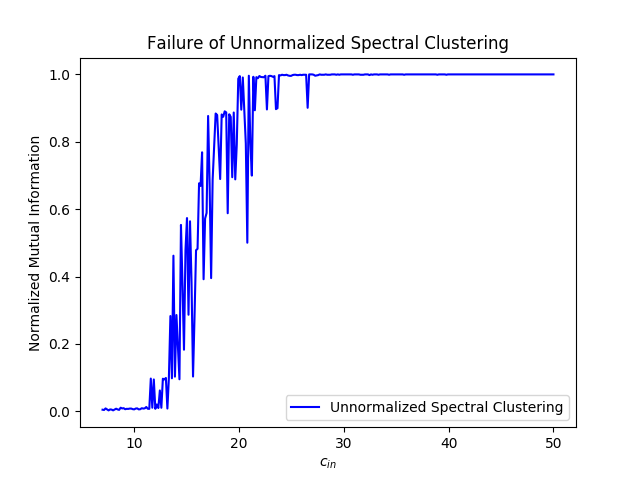
\includegraphics[width=14cm]{figures/spec_fail.png}
\end{center}
   \caption[Failure of spectral clustering]{Failure of spectral clustering. We fixed the value $c_\text{out} = 1$, and, for each of the three hundred values of $c_\text{in}$ equally spaced in the interval going from $7$ to $50$,  we used the stochastic block model to construct a graph of order $m = 10000$ ten times (with parameter $k=2$). Then we used unnormalized spectral clustering to cluster each of the graphs and computed the normalized mutual information (measure which will be explained in Chapter~\vref{numexp}) of the results. In the graph, we show the average of the ten values NMI for each value of $c_\text{in}$. The horizontal axis represents the value of $c_\text{in}$ and the vertical axis represents the normalized mutual information of the set of clusters found by the unnormalized spectral clustering.}
   \label{spec_fail}
\end{figure}

% Why does that happen? Semicircle law (cite paper) (maybe show figure if there is enough time)
The reason for this failure is as follows: as we have seen in the ideal approach for deriving spectral clustering, the algorithm needs to find the eigenvectors corresponding to the $k$ eigenvalues with the largest absolute value.
However, in random graphs such as those generated by SBM, ``phantom'' eigenvalues might invade this group of $k$ eigenvalues, yielding problematic eigenvectors which give rise to wrong labels.
Eugene Wigner gave a asympotic bound in 1958 \cite{circle} for the random part of the spectrum of the adjacency matrix of such graphs, which become known as \textit{Wigner's semicircle law}. 
For the SBM with the parameters we have discussed, the law states that when $m \rightarrow \infty$, the following holds:
\begin{equation} \label{circle_equation}
   \mathbb P (\lambda) = \frac{1}{2 \pi c} \sqrt{4c - \lambda^2},
\end{equation}
where $\mathbb P (\lambda)$ denotes the probability that $\lambda \in \mathbb R$ is an eigenvalue.
When the difference $c_\text{in} - c_\text{out}$ becomes closer to the theoretical limit, the relevant largest eigenvalues get closer to semicircle given by Equation~\vref{circle_equation}.
And since $m$ is never really gets to infinity, any little disturbance in Wigner's law may cause a phantom eigenvalue invasion to disturb the algorithm.

% A solution: using Bethe Hessian (define it and say what value of r to use)
To deal with this issue, Alaa Saade et al. devised a new way of performing spectral clustering in \cite{bethe} which is effective even close to the theoretical limit. 
Instead of the unnormalized Laplacian or normalized Laplacian we have discussed before, this new algorithm uses the so called \textit{Bethe Hessian matrix} $H \in \mathbb R ^{m \times m}$ to perform clustering:
\begin{equation}\label{bethe_definition}
   H(r) = (r^2 - 1) E_m -r A + D.
\end{equation}

Here, $E_m \in \mathbb R^{m \times m}$ denotes the identity matrix of order $m$, $A \in \mathbb R^{m \times m}$ denotes the adjacency matrix of the (unweighted) graph considered, $D \in \mathbb R^{m \times m}$ denotes the diagonal matrix whose $D_{ii}$ elements are given by the sum of the elements of the matrix $A$'s $i$-th row, for each $i \in \Iintv{1,m}$ and $r \in \mathbb R$ is a parameter.
% Best value of r for general matrix: r = sqrt(rho(A)), where rho(A) is the spectral radius of the non-backtracking operator
The best value of $r$ for matrices generated by the SBM is known to be $\sqrt{c}$.
For general adjacency matrices, it is known to be $r = \sqrt{\rho {(A)}}$, where $\rho (A)$ denotes the \textit{spectral radius} of the matrix $A$.
The justification of why the Bethe Hessian works, and why those values of the parameter $r$ are appropriate can be found in \cite{bethe}.

\begin{algorithm}
\caption{Bethe Hessian spectral clustering}\label{bethe_clustering}
\begin{algorithmic}[1]
   \Require 
      \Statex Adjacency Matrix of the graph $G = (V,E)$: $A \in \mathbb R ^ {m \times m}$ 
      \Statex Number of Clusters: $k \in \mathbb Z_{>1}$
      \Statex Parameter for Bethe Hessian: $r \in \mathbb R$
   \Ensure 
      \Statex Partition of the set of vertices $V$: $\{ C_1, C_2, \cdots, C_k \} \subseteq V$
      \vspace{0.2 cm}
   \State Compute the Bethe Hessian $H(r)$ of $A$ as described in Equation~\vref{bethe_definition}.
   \State Compute the first $k$ eigenvectors $(x_1, x_2, \cdots, x_k) \in (\mathbb R^{m})^k$ of $H(r)$.
   \State Let $X \in \mathbb R^{m \times k}$ be the matrix containing the vectors $x_1, x_2, \cdots, x_k$ as columns.
   \State Form the matrix $Y \in \mathbb R^{m \times k}$ by normalizing the columns of $X$.
   \State Let $(y_1, y_2, \cdots, y_m) \in ( \mathbb R^{1 \times k} )^m$ represent the row-vectors of $Y$.
   \State Cluster $(y_1, y_2, \cdots, y_m)$ using $k$-means into clusters $\{ D_1, D_2, \cdots, D_k \} $.
   \State For each $i \in \Iintv{1,k}$, set $C_i = \{ v_j \in V: y_j \in D_i \}$.
\end{algorithmic}
\end{algorithm}


% for reference, Bethe Hessian for weighted case (maybe do experiment next week)
A problem with the definition of Bethe Hessian matrix we have given in Equation~\vref{bethe_definition} is that it is only valid when the graph is unweighted.
For reference, we will also provide the Bethe Hessian matrix of weighted graphs $H_G(r) \in \mathbb R^{m \times m}$ below. For all $(i,j) \in \Iintv{1,m}^2$, we have:
\begin{equation}
   \left( H_G(r) \right)_{ij} = \delta _{ij} \left( 1 + \sum _{k \in \partial v_i}\frac{{A_{ij}}^2}{r^2 - {A_{ik}}^2} \right) - \frac{r A_{ij}}{r^2 - {A_{ij}}^2},
\end{equation}
where $\delta_{ij}$ denotes the Kronecker delta and $\partial i$ denotes the set of neighbors of $v_i$.


%-----------------------------------------------------------------

\chapter{Constrained spectral clustering with FAST-GE-2.0}\label{fastge2chapter}

% Introduction
The Information Age has brought with it large incentives to organize and process big amounts of data.
Traditionally, two main approaches have been used to deal with this task: classification and clustering.
While classification is widely used in situations where training data is abundant, such as recommendation systems, spam detection and speech recognition, this class of methods is not applicable to unlabeled datasets, which have been traditionally handled by clustering algorithms.
However, since clustering only makes use of the internal structure of the data, our control over the process is limited.
In this context, a new class of semi-supervised algorithms known as constrained clustering has appeared.
While these methods do not demand large amounts of labeled data as inputs, they still make it possible for a small amount of training data to influence the final outcome of the clustering process.
In this chapter, we describe FAST-GE-2.0, a spectral way of performing constrained clustering and see the theory behind its correctness.
This chapter is mainly a survey of the results from \cite{fastge2}, although we have changed some of the presentation and notation as to make them fit better with the rest of this thesis, supplied some additional explanations and justifications not present in the original paper and provided some new results that connect to the rest of the thesis.\footnote{For example, Figure~\vref{gm}, Figure~\vref{gh}, Proposition~\vref{spanOfLn}, Proposition~\vref{spanOfLh} and Proposition~\vref{huesing}.}

\section{Constrained Clustering}
In this chapter, $m$, $n$, and $k$ represent positive integers, with $k > 1$.

% What is Constrained Clustering? Why is it important? Where is it used?
Given a dataset $\mathcal D \subseteq \mathbb{R}^{n }$ (or equivalently a weighted graph $G = (V,E)$ of order $m$) and a set of contraints, to perform constrained clustering on the data means to find a proper partition $(C_1, C_2, \cdots, C_k)$ of $V$ such that:
\begin{itemize}
   \item For all $i \in \Iintv{1,k}$, edges of vertices in the same subset $C_i$ have big weights.
   \item For all $(i,j) \in \Iintv{1,k}^2$, edges of vertices in different subsets $C_i$ and $C_j$ have small weights.
   \item Constraints are followed as much as possible.
\end{itemize}

These constraints are usually small in number and represent whether certain groups of vertices should forcibly stay together or forcibly stay apart.
For example, in image segmentation, one of the main applications of constrained spectral clustering, a user selects a small amount of points in an image that she believes should stay in the same segment (e.g. points of a uniform background, or points of a tree). Then the contrained clustering algorithm tries to divide the image in segments (clusters) such that the points selected by the user stay in the same segment.


% How are constraints going to be represented in this chapter (FAST-GE-2.0)
There are several ways of representing these constraints, each leading to different algorithms. 
In this thesis we will work with must-link constraints (ML) and cannot-link constraints (CL) encoded as follows:

A set of constraints is given by $k$ disjoint subjects of $V$,
\begin{equation}
   \{ V_1, V_2, \cdots, V_k \} \subseteq V,
\end{equation}
such that: (1) for all $i \in \Iintv{1,k}$, if $(u,v) \in {V_i}^2$ then there exists a ML contraints between the vertices $u$ and $v$; and (2) for all $(i,j) \in \Iintv{1,k}^2$, if $(u,v) \in V_i \times V_j$ and $i \ne j$ then there exists a CL contraint between the vertices $u$ and $v$. 

An algorithm we may eventually develop, then, must be set up in such a way that violations of ML and CL constraints (such as, e.g., two vertices in different constraint sets $V_1$ and $V_2$ being in the same cluster $C_1$) have a negative effect on its effort to satisfy the objective function.

\section{FAST-GE-2.0}
We will now discuss FAST-GE-2.0, a spectral algorithm proposed by Chengming Jiang, et al, for constrained clustering in \cite{fastge2}.
% What is the objective of a p-way contrained clustering (slide; no equation)
We are given a fully connected graph $G = (V,E)$ of order $m$ with adjacency matrix $A$.
Assume a set of constraints $\{V_1, V_2, \cdots, V_k \}$ is given.
The objective of FAST-GE-2.0, in line with our discussion in the last section, is to find a proper partition $(C_1, C_2, \cdots, C_k)$ of $V$ such that $V_i \subseteq C_i$ for all $i \in \Iintv{1,k}$, where, for each pair $(i,j) \in \Iintv{1,m}^2$, vertices $(u,v) \in {C_i}^2$ have edges with high weight and vertices $(u,v) \in {C_i} \times {C_j}$, with $i \ne j$ have edges with low weight.
FAST-GE-2.0 manages to satisfy these constraints indirectly by using auxiliary graphs and encoding the ML and CL constraints into the Laplacian matrices dealth with in the algorithm.

\subsection{Auxiliary graphs}
In this subsection we define the auxiliary graphs used in FAST-GE-2.0.

% Graph G_M (include figure)
\subsubsection*{The graph $G_M$}

\begin{definition}
   The graph $G_M = (V,E)$ is defined by its adjacency matrix 
   \begin{equation}\label{am}
   A_M = \sum_{\ell = 1}^k A_{M_{\ell}},
\end{equation}
   where, for each $(\ell, i, j) \in \Iintv{1,k} \times \Iintv{1, m}^2$, the entries of the submatrix $A_{M_{\ell}} \in \mathbb R^{m \times m}$ are given by:
   \begin{equation}
      (A_{M_{\ell}})_{ij} =
      \begin{cases}
         (d_i d_j) / (d_{\min} d_{\max}), & \text{ if $(v_i, v_j) \in {V_{\ell}}^2$} \\
         0, & \text{ otherwise.}
      \end{cases}
\end{equation}
Here, for each $i \in \Iintv{1,m}$, $d_i$ represents the degree of the vertex $v_i$. 
Futhermore, $d_{\min}$ and $d_{\max}$ represent the smallest and biggest element of the set $\{ d_i \}_{i=1}^m$, respectively.
\end{definition}

As shown in Figure~\vref{gm}, if we define $G_M$ as above, for any given $\ell \in \Iintv{1,k}$, the quantity
\begin{equation}
   \cut_{G_M\,}(C_{\ell}) = \sum_{\substack{v_i \in C_{\ell} \\ v_j \overline{C_{\ell}}}} (A_M)_{ij} 
\end{equation}
%measures the amount of violations of ML constraints relative to the cut of $C_{\ell}$.
measures the degree to which the proper partition $(C_1, C_2, \cdots, C_k)$ violates the ML constraints.
Therefore we must try to minimize it as much as possible.

\begin{figure}
\begin{center}
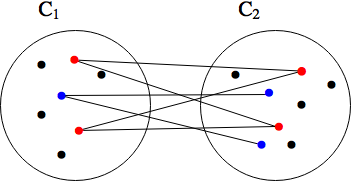
\includegraphics[width=8cm]{figures/gm.png}
\end{center}
   \caption[Graphical representation of $\cut_{G_M\,}(C_1)$ for a simple graph $G=(V,E)$]{Graphical representation of $\cut _{G_M\,}(C_1)$ for a simple simple graph $G = (V,E)$.  In this example, red vertices are elements of $V_1$, blue vertices are elements of $V_2$ and black vertices are elements of $V \setminus (V_1 \cup V_2)$. The black lines represent elements of $A_M$ that contribute to the amount of violations of ML given by $\cut _{G_M\,}(C_1)$. Note that all non-zero elements of $A_M$ must connect vertices of the same color, and all terms contributing to $\cut _{G_M\,}(C_1)$ must connect vertices in different clusters; hence the lines in the figure. We want elements of the same color to stay in the same cluster as much as possible. Therefore, we must try to decrease the amount of black lines.}
\label{gm}
\end{figure}

% Graph G_H (include figure)
\subsubsection*{The graph $G_H$}

\begin{definition}
The graph $G_H = (V,E)$ is defined by its adjacency matrix
   \begin{equation}\label{ah}
      A_H = \frac{1}{m} \, (A_C + {A_C}^T + A_K).
   \end{equation}
   Here, $A_C \in \mathbb{R}^{m \times m}$ is a matrix whose values are given by
   \begin{equation}
      (A_C)_{ij} = 
      \begin{cases}
      (d_i d_j)/(d_{\min} d_{\max}), & \text{ if $(v_i, v_j) \in V_{\ell_1} \times V_{\ell_2}$ and $\ell_1 \ne \ell_2$} \\
         0, & \text{ otherwise,}
      \end{cases}
   \end{equation}
   for each $(\ell_1, \ell_2, i, j) \in \Iintv{1,k}^2 \times \Iintv{1,m}^2$. 
   For all $i \in \Iintv{1,m}$, $d_i$ represents the degree of the vertex $v_i$. $d_{\min}$ and $d_{\max}$ represent the smallest and biggest element of the set $\{ d_i \}_{i=1}^m$, respectively.
   Furthermore, $A_K \in \mathbb{R}^{m \times m}$ is a matrix whose entries are given by 
   \begin{equation}
      (A_K)_{ij} = \frac{  \left( d^{(K)} \right) _i \cdot \left( d^{(K)} \right) _j }{ \sum_{p = 1}^m (d^{(K)})_p },
   \end{equation}
   for each $(i,j) \in \Iintv{1,m}^2$. Here, for every $i \in \Iintv{1,m}$, $\left( d^{(K)} \right) _i$ represents the sum of the elements in the $i$-th column of the matrix $A_C + {A_C}^T$.
\end{definition}

As shown in Figure \vref{gh}, if we define $G_H$ as above, for any given $\ell \in \Iintv{1,k}$, the quantity
\begin{equation}
   \cut _{G_H \,} (C_{\ell}) = \sum_{\substack{v_i \in C_{\ell} \\ v_j \in \overline{C_{\ell}}}} (A_H)_{ij} 
\end{equation}
measures the degree to which the proper partition $(C_1, C_2, \cdots, C_k)$ satisfies the CL constraints (as long as we do not consider $A_K$). 
Therefore we must try to maximize it as much as possible.

\begin{figure}
\begin{center}
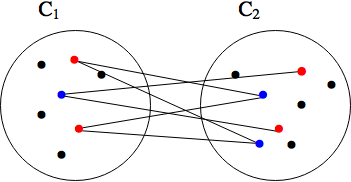
\includegraphics[width=8cm]{figures/gh.png}
\end{center}
   \caption[Graphical representation of $\cut_{G_H\,}(C_1)$ for a simple graph $G=(V,E)$]{Graphical representation of $\cut _{G_H\,}(C_1)$ for a simple simple graph $G = (V,E)$.  In this example, red vertices are elements of $V_1$, blue vertices are elements of $V_2$ and black vertices are elements of $V \setminus (V_1 \cup V_2)$. The black lines represent elements of $A_C$ that contribute to the amount obedience of CL given by $\cut _{G_H\,}(C_1)$. Note that all non-zero elements of $A_C$ must connect vertices of different colors, and all terms contributing to $\cut _{G_H\,}(C_1)$ must connect vertices in different clusters; hence the lines in the figure. We want elements of different colors to stay in the different clusters as much as possible. Therefore, we must try to increase the amount of black lines.}
\label{gh}
\end{figure}

The matrix $A_K$ is called a \textit{demand matrix}, and it is used in the construction of the graph $G_H$ in order to obtain some guarantees related to the spectral relaxation of FAST-GE-2.0. 
The mathematical details behind its use are beyond the level of this thesis.
More details about it can be found in \cite{fastge1}.


\subsection{Objective function}
In this and the following subsections, we assume $\ell \in \Iintv{1,k}$.

% Measure of badness
From our discussions on the last section, we know that we want to both minimize $\cut _{G_M\,}(C_{\ell})$ and to maximize $\cut _{G_H\,}(C_{\ell})$.
A natural next step, then, is to create some form of measure involving both cuts that we can optimize.

\begin{definition}
  We define the measure of badness $\phi_\ell$ relative to a cluster $C_\ell$ as follows:
   \begin{equation}
      \phi_\ell = \frac{\cut_{G_M\,} (C_\ell) + \cut_{G\,}(C_\ell)}{\cut_{G_H\,}(C_\ell)},
   \end{equation}
   where $G$ is the original graph we are trying to cluster with adjacency matrix $A$.
\end{definition}

Note that from our discussion in the past section, the only way to minimize $\phi_\ell$ is to either
\begin{enumerate}[(a)]
   \item minimize $\cut_{G_M\,}(C_\ell)$, which is the same as minimizing the amount of violations of ML constraints; or to
   \item minimize $\cut_{G\,}(C_\ell)$, which is the same as selecting a better cluster $C_\ell$ from the point of view of pure clustering; or to
   \item maximize $\cut_{G_L\,}(C_\ell)$, which is the same as maximizing the amount of obedience to CL constraints.
\end{enumerate}

Therefore, for any given cluster $C_\ell$, the measure $\phi_\ell$ successfully encapsulates all of our objectives in constrained clustering.

\begin{remark}
   The value $\cut_{G_M\,}(C_\ell) + \cut_{G\,}(C_\ell)$ may be expressed equivalently by $\cut_{G_N\,}(C_\ell)$, where $G_N$ is a \textit{new} graph defined by its adjacency matrix:
   \begin{equation}
      A_N = A_M+A.
   \end{equation}
   We can then write the measure of badness $\phi_\ell$ as
   \begin{equation}
      \phi_\ell = \frac{\cut_{G_N\,}(C_\ell)}{\cut_{G_H\,}(C_\ell)}.
   \end{equation}
\end{remark}

% Get the equation for k-way constrained partioning

\begin{definition}
   The \textit{objective of FAST-GE-2.0} for a $k$-way constrained partitioning is given by
   \begin{equation}\label{objective}
      \min_{(C_1, C_2, \cdots, C_k)} \max_{\ell} \, \phi _\ell.
   \end{equation}
   In other words, we want to find a proper partition $(C_1, C_2, \cdots, C_k)$ of $V$ that minimizes the biggest value of $\phi_\ell$ for all clusters $C_\ell$.
\end{definition}

\subsection{Eigenproblem formulation}
In this subsection, we will analyze the case where $k = 2$ as it was done in \cite{fastge2}.
An analysis of the general case, which may be found in \cite{fastge1}, requires linear algebra knowledge not expected from the main audience of this thesis, so we omit it.

% Refer to theorem to say the equation above is the same as Rayleigh quotient
In the case $k=2$, if we set $C_1 = C$ and $C_2 = \overline C$, the objective function given in Equation \vref{objective} can be rewritten as 
\begin{equation}\label{phi2}
   \min_C \frac{\cut_{G_N\,}(C)}{\cut_{G_H\,}(C)}.
\end{equation}

Here, Theorem \vref{xtxcut} allows us to rewrite Equation \vref{phi2} in more convenient terms. 
An important point to note, however, is that since the $\vol (V)$ is constant, we can ignore it in the optimization analysis.
The objective function becomes then:
\begin{equation}
   \min_{{x_C}^TL_H {x_C} \ne 0} \frac{{x_C}^TL_N{x_C}}{{x_C}^TL_H{x_C}},
\end{equation}
where $L_N$ and $L_H$ are respectively the unnormalized Laplacians of the graphs $G_N$ and $G_H$, and where $x_C$ is an indicator vector as defined in Equation~\vref{indicator}.

% Problem is NP-complete (reference to somewhere that proves it --> check paper)
With a similar argument as the one used for Equation~\vref{npequation}, one can prove that the optimization problem above is NP-complete \cite{fastge2}.
% Approximation
It stands to reason then to perform spectral relaxation and try to apply the General Courant-Fischer Min-Max Theorem to the objective function as we did for regular spectral clustering. The function becomes:
\begin{equation}\label{inf}
   \inf_{\substack{x \in \mathbb R^m \\ x^T L_H x \ne 0}} \frac{x^T L_N x}{x^T L_H x},
\end{equation}
where $x \in \mathbb R^{m }$ is now an arbitrary real column-vector.
Note that we have written $\inf$ instead of $\min$.
The reason for this is that the minimum is not guaranteed to be achieved.

Even after performing the spectral relaxation above, however, we still cannot be sure we are allowed to apply General Courant-Fischer, since it requires not only that the Laplacian $L_H$ in the denominator be positive semidefinite (which is true by Corollary \vref{unnormalizedLaplacianProperties}), but also that $\mathcal N (L_H) \subseteq \mathcal N (L_N)$. 
Let us check whether this condition holds or not.


\begin{proposition} \label{spanOfLn}
   If $G$ is a connected graph, then 
   \begin{equation}
      \mathcal N (L_N) = \spn \{ 1_{m \times 1} \}.
   \end{equation}
\end{proposition}

\begin{proof}
   We known from the definition that $A_N = A + A_M$.
   Since $G$ is connected, all elements of $A$ are positive, and we can conclude that all elements of $A_N$ are also positive.
   Now assume $x \in \mathbb R ^{m}$ is an element of the nullspace of $L_N$, i.e. $L_N x = 0$.
   By Proposition \vref{xtlx}, we know that:
   \begin{equation*}
      x^T (L_N x) = \frac{1}{2} \sum_{i,j=1}^m (A_N)_{ij} (x_i - x_j)^2 = 0.
   \end{equation*}
   For all $(i,j) \in \Iintv{1,m}^2$, $(A_N)_{ij} > 0$, so we must have $x_i - x_j = 0$ for all these pairs.
   That is, all elements of $x$ must necessarily be the same. \qed
\end{proof}

\begin{proposition} \label{spanOfLh}
   Even if $G$ is connected, 
   \begin{equation}
      \mathcal N (L_H) \subseteq \mathcal N (L_N)
   \end{equation}
   does not necessarily hold.
\end{proposition}

\begin{proof}
   We will give a proof to this proposition by showing a connected graph $G$ for which $L_H$ has an eigenvector $x$ such that $x \notin \mathcal \spn \{ 1_{m \times 1} \}$. 
   Assume $G$ is the completely connected graph of order $m$ where $A_{ij} = 1$, for all $(i,j) \in \Iintv{1,m}^2$.
   Assume further that $V_1 = \{ v_1 \}$ and $V_2 = \{ v_2 \}$.
   We must have that $d_i = m(m-1)/2$, for all $i \in \Iintv{1,m}$, and thus, from the definitions given in this section:
   \begin{equation*}
      A_C = 
      \begin{bmatrix}
         0 & 1 & 0 & \cdots & 0 \\
         1 & 0 & 0 & \cdots & 0 \\
         0 & 0 & 0 & \cdots & 0 \\
         \vdots & \vdots & \vdots & \ddots & 0 \\
         0 & 0 & 0 & \cdots & 0 
      \end{bmatrix}.
   \end{equation*}
   We must have then that $\left( d^{(K)} \right) _1 = \left( d^{(K)} \right)_2 = 2$ and $\left( d^{(K)} \right)_i = 0$ for all $i \in \Iintv{3,m}$. Thus
   \begin{equation*}
      A_K =
      \begin{bmatrix}
         1 & 1 & 0 & \cdots & 0 \\
         1 & 1 & 0 & \cdots & 0 \\
         0 & 0 & 0 & \cdots & 0 \\
         \vdots & \vdots & \vdots & \ddots & 0 \\
         0 & 0 & 0 & \cdots & 0 
      \end{bmatrix},
      \text{ and }
      A_H = \frac{1}{m} \, (A_C + {A_C}^T + A_K) = 
      \begin{bmatrix}
         1/m & 3/m & 0 & \cdots & 0 \\
         3/m & 1/m & 0 & \cdots & 0 \\
         0 & 0 & 0 & \cdots & 0 \\
         \vdots & \vdots & \vdots & \ddots & 0 \\
         0 & 0 & 0 & \cdots & 0 
      \end{bmatrix}.
   \end{equation*}
   Finally, computing the Laplacian $L_H = D_H - A_H$, where $D_H = \text{diag} \,(4/m, 4/m, 0 \cdots, 0) \in \mathbb R^{m \times m}$ is the diagonal matrix of the graph:
   $G_H$:
   \begin{equation*}
      L_H =
      \begin{bmatrix}
         3/m & -3/m & 0 & \cdots & 0 \\
         -3/m & 3/m & 0 & \cdots & 0 \\
         0 & 0 & 0 & \cdots & 0 \\
         \vdots & \vdots & \vdots & \ddots & 0 \\
         0 & 0 & 0 & \cdots & 0 
      \end{bmatrix},
   \end{equation*}
   which clearly has $x = {\begin{bmatrix} 0 & 0 & 1 & 1 & \cdots & 1 \end{bmatrix}}^T \in \mathbb R ^{m} \setminus \spn \{ 1_{m \times 1} \}$ as one of its eigenvectors. \qed
\end{proof}

Proposition \vref{spanOfLh} shows to us then that we cannot use the Generalized Courant-Fischer Theorem as a guarantee that the spectral relaxation will work.
Fortunately, Chengming Jiang et al. proved the following theorem in \cite{fastge2}.

\begin{theorem}
   \label{fastge2theorem}
   For the matrices $L_N$ and $L_H$ defined in this chapter, the following holds
   \begin{enumerate}[(a)]
      \item the pencil $(L_N, L_H)$ has $r$ finite non-negative generalized eigenvalues $0 \le \lambda_1 \le \lambda_2 \le \cdots \le \lambda_r$, where $r$ denotes the rank of the matrix $L_H$.
      \item For every $i \in \Iintv{1,r}$, the following holds
         \begin{equation}
            \lambda_i = \max_{\substack{\mathcal X \subseteq \mathbb R^m \\ \dim {\mathcal X} = n-i+1 }} \min_{\substack{x \in \mathcal X \\ x^T L_H x > 0}} \frac{x^T L_N x}{x^T L_H x}.
         \end{equation}
         In particular, 
         \begin{equation}
            \lambda_1 = \min_{\substack{x \in \mathbb R^m \\ x^TL_Hx>0}} \frac{x^tL_N x}{x^T L_H x}.
         \end{equation}
   \end{enumerate}
\end{theorem}

Item (b) of Theorem \vref{fastge2theorem} guarantees to us that the $\inf$ in Equation \vref{inf} can be substituted by a $\min$:
\begin{equation}\label{min}
   \min_{\substack{x \in \mathbb R^m \\ x^T L_H x \ne 0}} \frac{x^T L_N x}{x^T L_H x},
\end{equation}
and that this minimum is given by the smallest finite eigenvalue of the following generalized eigenvalue problem:
\begin{equation}\label{generalizedEigenproblem}
   L_N x = \lambda L_H x.
\end{equation}

Our problem, then, is reduced to solving the generalized eigenproblem given by Equation \vref{generalizedEigenproblem}, a particular case of the well-studied Generalized Hermitian Eigenvalue problem.
Several approaches exist to solve it: Direct methods, Lanczos methods and Locally Optimal Block Preconditioned Conjugate Gradient (LOBPCG) algorithm, for example. 
However, all of them require that the pencil $(L_N, L_H)$ be non-singular (see \cite{templates}).
In other words, we need the following condition to hold for all $\lambda \in \mathbb R$:
\begin{equation}
   \det (L_N - \lambda L_H) \ne 0,
\end{equation}
which is problematic due to the following proposition:

\begin{proposition} \label{huesing}
   The pencil $(L_N, L_H)$ is singular.
\end{proposition}

\begin{proof}
   Since $1_{m \times 1}$ is in the nullspace of both $L_N$ and $L_H$ (Corollary \vref{unnormalizedLaplacianProperties}), we know that, for any $\lambda \in \mathbb R$,
   \begin{equation*}
      (L_N - \lambda L_H) 1_{m \times 1} = L_N 1_{m \times 1} - \lambda L_H 1_{m \times 1} = 0 - \lambda 0 = 0 = 0 \, 1_{m \times 1}.
   \end{equation*}
   Therefore, the matrices $(L_N - \lambda L_H)$ have $0$ as an eigenvalue and are, therefore, singular. \qed
\end{proof}

% Regularization (theorem 2 from paper)
To fix this problem, then, we need to regularize the pencil $(L_N, L_H)$.
The following theorem, also proved in \cite{fastge2}, allows us to do that:

\begin{theorem}
   Suppose the pencil $(L_N, L_H)$ has the finite eigenvalues $\lambda_1 \le \lambda_2 \le \cdots \le \lambda_r$, where $r$ is the rank of the matrix $L_H$. Let
   \begin{equation}\label{regularization}
      K = - L_H,  \text{ and } M = L_N + \mu L_H + ZSZ^T,
   \end{equation}
   where $Z \in \mathbb R^{m \times s}$ is an orthonormal basis of the common nullspace of $L_N$ and $L_H$, $S \in \mathbb R ^{s \times s}$ is an arbitrary positive definite matrix, and $\mu \in \mathbb R$.
   Then the following holds:
   \begin{enumerate}[(a)]
      \item the matrix $M$ is positive definite.
      \item the generalized eigenvalues of the pencil $(K, M)$ are $\sigma _1 \le \sigma_2 \le \cdots \le \sigma_r < \sigma_{r+1} = \sigma_{r+2} = \cdots = \sigma_m = 0$, where, for each $i \in \Iintv{1,r}$, $\sigma_i = -1/(\lambda_i + \mu)$.
   \end{enumerate}
\end{theorem}

The theorem above lets us compute the $k$ smallest eigenvalues $\{ \lambda_i \}_{i=1}^k$ of the generalized eigenproblem in Equation \vref{min} by computing the $k$ \textit{largest} eigenvalues of the following generalized eigenproblem:
\begin{equation}
K x = \sigma M x,
\end{equation}
which can effectively be solved by methods such as Lanczos and LOBPCG.

% Algorithm
Given the considerations above, we can write the spectral algorithm for constrained clustering FAST-GE-2.0 as follows:

\begin{algorithm}
\caption{FAST-GE-2.0}\label{fastge2alg}
\begin{algorithmic}[1]
   \Require 
      \Statex Number of Clusters: $k \in \mathbb Z_{>1}$
      \Statex Adjacency Matrix of the graph $G=(V,E)$: $A \in \mathbb R ^ {m \times m}$ 
      \Statex Constraint Sets: $\{ V_1, V_2, \cdots, V_k \} \subseteq V$
      \Statex Regularization Parameters: $\mu \in \mathbb R$, $Z \in \mathbb R ^{n \times s}$, $S \in \mathbb R ^{s \times s}$
   \Ensure 
      \Statex Partition of the set of vertices $V$: $\{ C_1, C_2, \cdots, C_k \} \subseteq V$
      \vspace{0.2 cm}

   \State Compute the graphs $G_M$ and $G_H$ with respective adjacency matrices $A_M$ and $A_H$ as indicated in Equation \vref{am} and Equation \vref{ah}.
   \State Compute the unnormalized Laplacians $L_N$ and $L_H$ of the graphs $G_N$ and $G_H$. Here the adjacency matrix of $G_N$ is given by $A + A_M$.
   \State Compute $k$ eigenvectors corresponding to the $k$ largest finite generalized eigenvalues of the pencil $(K,M)$ in Equation \vref{regularization}. Let $X \in \mathbb R ^{m \times k}$ be the matrix containing these eigenvectors as columns.
   \State Let $Y \in \mathbb R ^{m \times k}$ be the matrix $X$ with rows and columns normalized.
   \State Let $(y_1, y_2, \cdots, y_k) \in (\mathbb R^{1 \times k})^m$ represent the row-vectors of $Y$.
   \State Cluster $(y_1, y_2, \cdots, y_m)$ using $k$-means into the clusters $ \{ D_1, D_2, \cdots, D_k \}$.
   \State For each $i \in \Iintv{1,k}$, set $C_i = \{ v_j \in V: y_j \in D_i \}$.
\end{algorithmic}
\end{algorithm}

% (maybe) reference to future numerical experiment


\chapter{Proposed method} \label{proposed_chapter}
In this chapter, we describe the method that gives the name to this thesis --- namely, extending the Bethe Hessian spectral clustering algorithm which we have described in Chapter \ref{bethechapter} so it is able to perform constrained clustering.
We first explain the main idea to extend the algorithm to the cases we are interested in, enumerate possible problems that we believe may occur with the extension together with some of our hypotheses about these problems and finally give a formal description of our proposed method.

\section{Our idea}
In Chapter \ref{bethechapter} we described the SBM generative model and the label recovery problem associated with it, and explained that in circumstances where the value of $c_\text{in} - c_\text{out}$ (where $c_\text{in}$ and $c_\text{out}$ are parameters of the model) is very small, then normal spectral clustering is ineffective at solving the problem, even when other algorithms are known to be effective.
Then we introduced a new way of performing clustering, the so called Bethe Hessian spectral clustering, which improves the efficiency of spectral clustering considerably. 
However, as we will see in Chapter \ref{numexp}, even when we use this improved Bethe Hessian version of spectral clustering, when the value of $c_\text{in} - c_\text{out}$ is close to the theoretical limit for the recovering of the model labels, we get disappointing results.

On the other hand, in Chapter \ref{fastge2chapter}, we presented a generalization of the concept of clustering, the so called constrained clustering, which uses an arbitrary amount of learning data to ``help shape'' how the clustering is done and get a better output.
We then described a spectral way of performing this generalization, the FAST-GE-2.0 algorithm and explained the theory behind its use.

In this chapter, we try to get the best of both worlds. 
While it is known that getting good clustering results in graphs generated by SBM is difficult when the difference $c_\text{in} - c_\text{out}$ is smaller than or very close to the theoretical limit, would the situation be the same if we are provided with some of the true labels of a certain amount of the vertices? If not, how much learning data would we need to get considerably better results?
To answer this questions, we propose a new algorithm (or, strictly speaking, a group of three very similar algorithms) which mixes the approaches described in Chapter \ref{bethechapter} and Chapter \ref{fastge2chapter}.

Before that, let us address one point that may appear in the reader's mind at this moment: it would not be unnatural for one to try to apply FAST-GE-2.0 directly to the graphs generated by SBM close to the limit and check if we get better results than just using the Bethe Hessian.
Unfortunately, as we have seen in Chapter \ref{fastge2chapter}, the step of spectral relaxation in FAST-GE-2.0 requires that the Laplacian matrix satisfy a number of steps, one of them being that the graph is connected. Unfortunately, graphs generated by the sparse version of SBM we described in Chapter \ref{fastge2chapter} are almost never connected, so we have no guarantees that FAST-GE-2.0 works.
Testing the algorithm directly, we find out that an error often occurs in the eigenproblem solution step. We believe this is due to the fact that getting even one eigenvector wrong can cause the algorithm to halt.
Besides, even in the few cases where there are no errors, the algorithm does not give results considerably better than the ones given by normal spectral clustering.
We conclude, then, that applying FAST-GE-2.0 to graphs generated by SBM is not viable.

But what if there was a way to apply FAST-GE-2.0 without getting any wrong eigenvectors?
As we have seen before, this is possible if we use the Bethe Hessian matrix instead of the normal Laplacian.
Our approach then is to substitute the unnormalized Laplacian used in FAST-GE-2.0 by the Bethe Hessian.


In the FAST-GE-2.0 algorithm, we deal with two Laplacians ($L_N$ and $L_H$), but we do not know
\begin{enumerate}[(a)]
   \item which of these two Laplacians give out ``wrong'' eigenvectors due to the randomness in the graph generated by the SBM; or
   \item which of them would actually cause the algorithm to halt even if some of the eigenvectors are wrong.
\end{enumerate}
Therefore, in this thesis we take an experimental approach. We consider the following three possible cases:
\begin{enumerate}[(1)]
   \item Substite both $L_N$ and $L_H$ by Bethe Hessian matrices in FAST-GE-2.0,
   \item Substitute only $L_N$ by Bethe Hessian matrices in FAST-GE-2.0,
   \item Substitute only $L_H$ by Bethe Hessian matrices in FAST-GE-2.0,
\end{enumerate}
and check whether any of these approaches bear good results.
The answer to this enquiry can be checked in Chapter~\ref{numexp}.

\section{Problem with the degrees}
Before giving a description of the proposed algorithm, however, we need to deal with the issue of the degrees.
Since the graphs generated by SBM are very sparse, it happens very often that some vertices will be isolated and will, therefore, have degree equal to $0$.

On the other hand, in FAST-GE-2.0, when we compute the adjacency matrix of the graphs $G_M$ and $G_H$ we must divide some elements by $d_\text{min}$.
If there is any isolated vertex, then, a division by $0$ will occur and the algorithm will halt.
While we believe there are many ways of dealing with this problem, we have chosen the simple approach of adding a loop (an edge that connects a vertex to itself) to all vertices in the graph.
That way, all vertices will have degree at least $1$ and no division by $0$ will occur.

We know that adding such edges will not affect the results structure of the graph because, for one thing, this transformation is isonomic in relation to all vertices.
Furthermore, the cluster structures themselves are not affected in the least because there will be no new edges connecting vertices that were in different clusters before the transformation.

\section{Algorithm}
Given the considerations discussed in this chapter, we provide the proposed algorithm in this section.
Here, each matrix each of $P_N$ and $P_H$ can be either a Bethe Hessian matrix or a unnormalized Laplacian matrix, as discussed in the previous section.

\begin{algorithm}
\caption{Proposed method: modified FAST-GE-2.0}\label{proposed_algorithm}
\begin{algorithmic}[1]
   \Require 
      \Statex Number of Clusters: $k \in \mathbb Z_{>1}$
      \Statex Adjacency Matrix of the graph $G=(V,E)$: $A \in \mathbb R ^ {m \times m}$ 
      \Statex Constraint Sets: $\{ V_1, V_2, \cdots, V_k \} \subseteq V$
      \Statex Regularization Parameters: $\mu \in \mathbb R$, $Z \in \mathbb R ^{n \times s}$, $S \in \mathbb R ^{s \times s}$
   \Ensure 
      \Statex Partition of the set of vertices $V$: $\{ C_1, C_2, \cdots, C_k \} \subseteq V$
      \vspace{0.2 cm}
   \State Perform the transformation $A \longmapsto A + E_m$ in order to solve the problem with degrees.
   \State Compute the graphs $G_M$ and $G_H$ with respective adjacency matrices $A_M$ and $A_H$ as indicated in Equation \vref{am} and Equation \vref{ah}.
   \State Compute the matrices $P_N$ and $P_H$ (as indicated in this and the past sections) of the graphs $G_N$ and $G_H$. Here the adjacency matrix of $G_N$ is given by $A + A_M$.
   \State Compute $k$ eigenvectors corresponding to the $k$ largest finite generalized eigenvalues of the pencil $(K,M)$ in Equation \vref{regularization}. Let $X \in \mathbb R ^{m \times k}$ be the matrix containing these eigenvectors as columns.
   \State Let $Y \in \mathbb R ^{m \times k}$ be the matrix $X$ with rows and columns normalized.
   \State Let $(y_1, y_2, \cdots, y_k) \in (\mathbb R^{1 \times k})^m$ represent the row-vectors of $Y$.
   \State Cluster $(y_1, y_2, \cdots, y_m)$ using $k$-means into the clusters $ \{ D_1, D_2, \cdots, D_k \}$.
   \State For each $i \in \Iintv{1,k}$, set $C_i = \{ v_j \in V: y_j \in D_i \}$.
\end{algorithmic}
\end{algorithm}



\chapter{Numerical experiments} \label{numexp}
In this chapter, we will present the descriptions and results of the experiments done in order to test the efficacy of the methods presented in the thesis. 
Before that, however, we need to explain how we can measure how good a partition obtained by a clustering algorithm is.

\section{Clustering evaluation and computing environment}
There is a very big number of ways of evaluating how good the output of a clustering method is.
These evaluating benchmarks can be divided in two types: internal evaluation, which is based exclusivily on the data that was clustered; and external evaluation, in which results are evaluated based on data not present in the data clustered, such as known labels.
External evaluation requires data that is not always necessarily available, so it is sometimes impossible to use it.
However, all the experiments done in this thesis use data that is accompanied by true class labels, so we can always use that kind of evaluation.

Mutual information is an external method to evaluate how good a clustering partition is based on information theory.

\begin{definition}
   Given a graph $G = (V,E)$ of order $m$ to be clustered, the \textit{mutual information} $\ii (C, T)$ of $C$ and $T$ is the measure that takes the set of clusters found by the algorithm $C = \{ C_1, C_2, \cdots, C_k \}$ and the set of clusters found by the algorithm $T = \{ T_1, T_2, \cdots, T_\ell \}$ and outputs a real number as follows:
\begin{equation}
   \ii (C, T) = \sum_{i=1}^k \sum _{j=1}^\ell \frac{|C_i \cap T_j|}{m} \log \left( \frac{m |C_i \cap T_j|}{|C_i| |T_j|} \right),
\end{equation}
where $|A|$ is the denotes the number of elements of the finite set $A$.
\end{definition}

This value has a nice probabilistic interpretation and measures how much information the presence or absence of each element in $C$ contributes to making the correct classification decision. 
We can say that the higher the value $\ii (C, T)$ is, the better the clusters found by the clustering algorithm.
The mutual information is $0$ when, for all $(i,j) \in \Iintv{1,k} \times \Iintv{1,\ell}$, $|C_i \cap T_j| = 0$ and it achieves its maximum value when $C$ perfectly recreates the classes of $T$.
However, $\ii (C,T)$ is also maximum whenever $C$ is subdivided in smaller clusters.
This is not desirable for us since we want the set of clusters to be as small as possible.
To solve this problem we need to perform some kind of normalization.
But before doing that we need to give a preliminary definition:

\begin{definition}
   Given a set of clusters $C = \{C_1, C_2, \cdots, C_k \}$ of a graph $G=(V,E)$ of order $m$, we define the \textit{entropy} of $C$ as the following quantity:
\begin{equation}
   \h (C) = - \sum_{i=1}^k \frac{|C_i|}{m} \log \left( \frac{|C_i|}{m} \right) .
   \end{equation}
\end{definition}

Entropy is a important concept in the field of information theory and measures the amount of disorder in the set of clusters $C$.  

With that definition in hands, we can then normalize the mutual information measure to avoid the problem we discussed.

\begin{definition}
   Given a graph $G = (V,E)$ of order $m$ to be clustered, the \textit{normalized mutual information} $\nmi (C, T)$ of $C$ and $T$ is the measure that takes the set of clusters found by the algorithm $C = \{ C_1, C_2, \cdots, C_k \}$ and the set of clusters found by the algorithm $T = \{ T_1, T_2, \cdots, T_\ell \}$ and outputs a real number as follows:
\begin{equation}
   \nmi (C,T) = \frac{2\ii (C,T)}{\h (C) + \h (T)}
\end{equation}
where $|A|$ is the denotes the number of elements of the finite set $A$.
\end{definition}

The two main properties of NMI we need to have in mind in this thesis are:

\begin{itemize}
   \item The higher the value of $\nmi (C,T)$, the better the set of clusters $C$ given by the algorithm.
   \item For any cluster sets $C$ and $T$ of any arbitrary graph, the value of $\nmi (C,T)$ is a number between $0$ and $1$. 
\end{itemize}

Therefore we can use NMI to evaluate how good the clusters given by any clustering algorithm are, and even compare the results of clustering in different graphs of different nature.
A more detailed account of NMI may be found in \cite{nmi}.

We show the computing environment used to perform the numerical experiments of this chapter in Table~\vref{environment}.

\begin{table}[h]
\centering
\caption{Computing environment used to perform the numerical experiments in this chapter}
\label{environment}
\begin{tabular}{l|l}
\hline
Operating system & macOS High Sierra 10.13.2 \\ \hline
Processor        & 2.2 GHz Intel Core i7     \\ \hline
Memory           & 8GB 1600 MHz DDR3         \\ \hline
Language         & Python (NumPy)            \\ \hline
\end{tabular}
\end{table}

\section{Experiment 1}
\subsection*{Objective}
The objective of this numerical experiment is to compare the performace of the Bethe Hessian spectral clustering algorithm with the performance of the unnormalized spectral clustering algorithm when clustering graphs generated by the stochastic block model.
\subsection*{Description}
For values of $c_\text{in}$ equally spaced in the interval $[7,25]$, with $c_\text{out} = 1$ fixed, we used the stochastic block model to construct ten graphs of size $m = 10000$ for two clusters ($q = 2$).
Then we used unnormalized spectral clustering and Bethe Hessian spectral clustering to cluster each of these graphs and computed the normalized mutual information of each of these sets of clusters.
Finally, we took the average of the NMI for each algorithm.

\subsection*{Results}
The results of this numerical experiment are shown in Figure~\vref{bethe_hessian_triumph}.

\begin{figure}[h]
\begin{center}
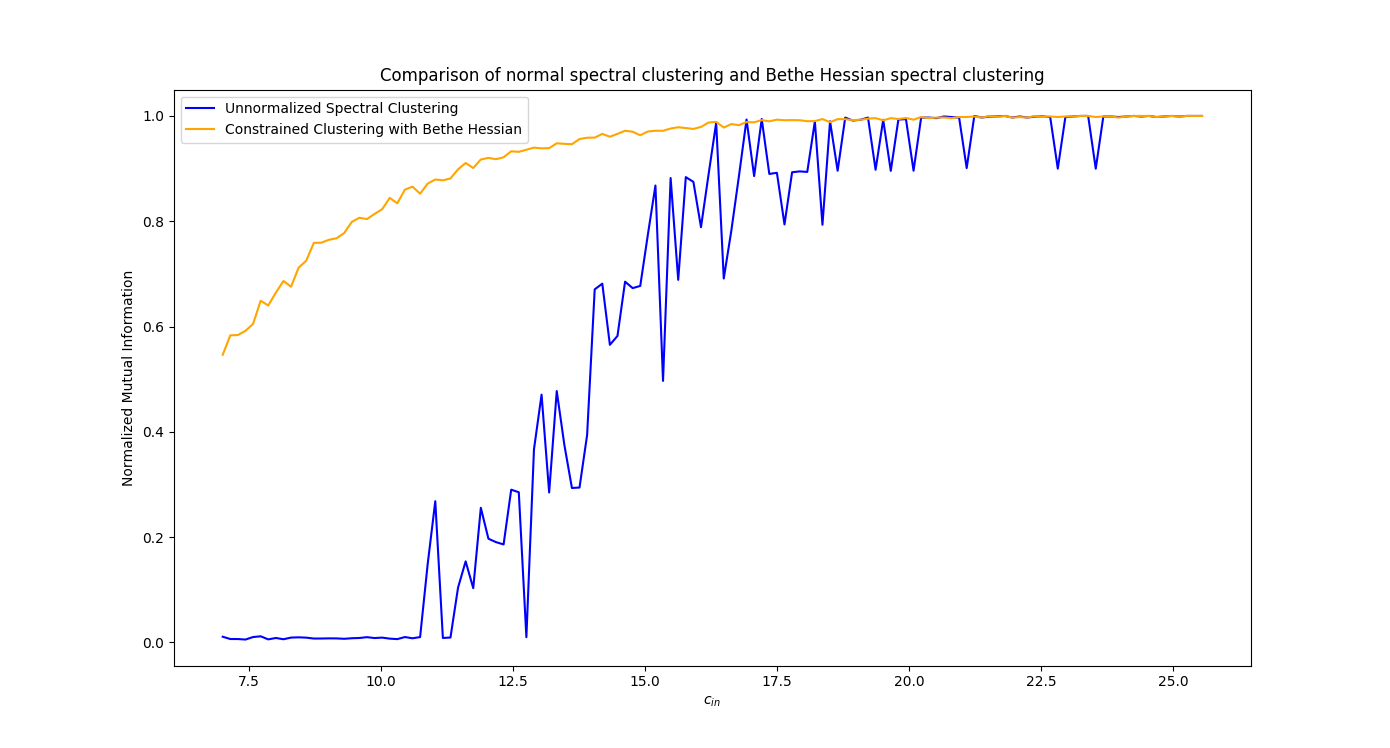
\includegraphics[width=14cm]{figures/bethe_hessian_triumph.png}
\end{center}
   \caption[Experimental results for clustering using unnormalized spectral clustering and Bethe Hessian clustering]{Experimental results for clustering using unnormalized spectral clustering and Bethe Hessian clustering. The horizontal axis represents the value of the parameter $c_\text{in}$ of the stochastic block generative model. The vertical axis represents the normalized mutual information of the set of clusters found by each algorithm and the true labels.}
\label{bethe_hessian_triumph}
\end{figure}

\subsection*{Discussion}
The results show that although unnormalized spectral clustering fails completely when $c_\text{in} - c_\text{out}$ is close to the theoretical limit, Bethe Hessian clustering has a much better performance. 
Furthermore, the range of values that Bethe Hessian clustering takes is much smaller than the ones for unnormalized clustering, even when $c_\text{in} - c_\text{out}$ is very big.
We can say, then, that the use of the Bethe Hessian for clustering graphs generated by SBM was a success.

\section{Experiment 2}
\subsection*{Objective}
The objective of the this numerical experiment is to compare the efficiency of the FAST-GE-2.0 algorithm we introduced in Chapter~\ref{fastge2chapter} with another non-spectral algorithm for constrained clustering, particularly in a case different from the ones discussed in \cite{fastge2}.
\subsection*{Description}
We used FAST-GE-2.0 for a semi-supervised clustering task and compared its efficiency with another semi-supervised clustering method: the constrained vector quantization error (CVQE) algorithm.
Ten features (one real, nine integers) were selected from the Statlog heart disease dataset.
The Gaussian similarity function $s_G: (x,y) \in (\mathbb R^{10})^2 \mapsto \exp ( - \norm{x-y}^2/2 \sigma ^2) \in \mathbb R$, where $\sigma = 5$, was used to construct the adjacency matrix $A$ of a fully connected graph of the data.
For the number of constraints $n_c = \left| \cup_{i=1}^k V_i \right|$ varying between $10$ and $280$, we used FAST-GE-2.0 and CVQE for constrained clustering.
For each value of $n_c$, we selected the elements of $\cup_{i=1}^k V_i$ randomly $10$ different times, and computed the average of the normalized mutual information of both methods.

\subsection*{Results}
The results of the experiment are shown in Figure~\vref{MR}.
For reference, we also provide the linear regression fit line and its 95\% confidence interval for each method's results.

\begin{figure}[h]
\begin{center}
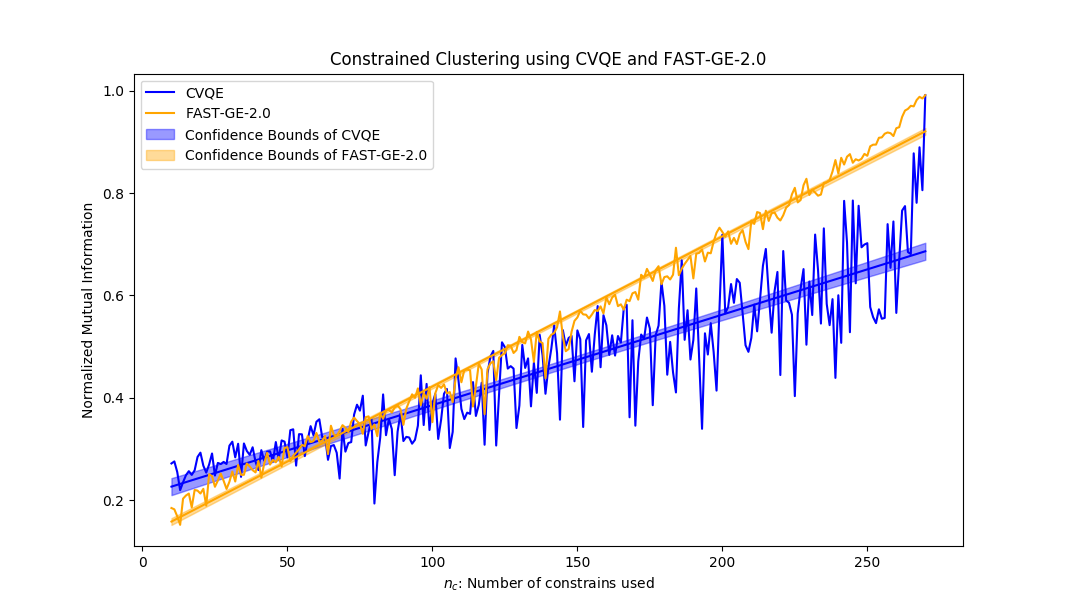
\includegraphics[width=14cm]{figures/MR.png}
\end{center}
   \caption[Experimental results for constrained clustering using FAST-GE-2.0 and CVQE]{Experimental results for constrained clustering using FAST-GE-2.0 and CVQE. The horizontal axis represents the number of constraints given to each algorithm and the vertical axis represents the normalized mutual information of the set of clusters found by each algorithm and the true labels.}
\label{MR}
\end{figure}

\subsection*{Discussion}
The results show that although the CVQE algorithm shows better results for $n_c < 80$, FAST-GE-2.0 is generally better.
Furthermore, it is clear to see from its smaller confidence bounds that FAST-GE-2.0's results exhibit less variance and the algorithm is thus more reliable.



\section{Experiment 3}
\subsection*{Objective}
The objective of this numerical experiment is
\begin{enumerate}[(1)]
   \item verify if the modified version of FAST-GE-2.0 proposed in Chapter~\ref{proposed_chapter} works or halts; and
   \item to find out which of the three variations of FAST-GE-2.0 discussed in Chapter~\ref{proposed_chapter} works the best; and
   \item to find out if any of these variations of FAST-GE-2.0 works better than the Bethe Hessian clustering algorithm and unnormalized clustering algorithm and, if so, how much better they do.
\end{enumerate}
\subsection*{Description}
In this experiment, we performed constrained clustering using five different methods: unnormalized clustering, Bethe Hessian clustering, modified FAST-GE-2.0: both $L_N$ and $L_H$, modified FAST-GE-2.0: only $L_N$, and modified FAST-GE-2.0: only $L_H$. 
For each value of the number of constraints $n_c$ varying between $200$ and $990$, we used the stochastic block model to construct ten graphs of size $m = 10000$ for two clusters ($q=2$). Then we used the five different methods to perform either constrained clustering (FAST-GE-2.0's modifications) or clustering (the rest), and computed the normalized mutual information of each of these sets of clusters.
Finally, we took the average of the NMI for each algorithm.

\subsection*{Results}
The results of this experiment are shown in Figure~\vref{CDV}.

\begin{figure}[h]
\begin{center}
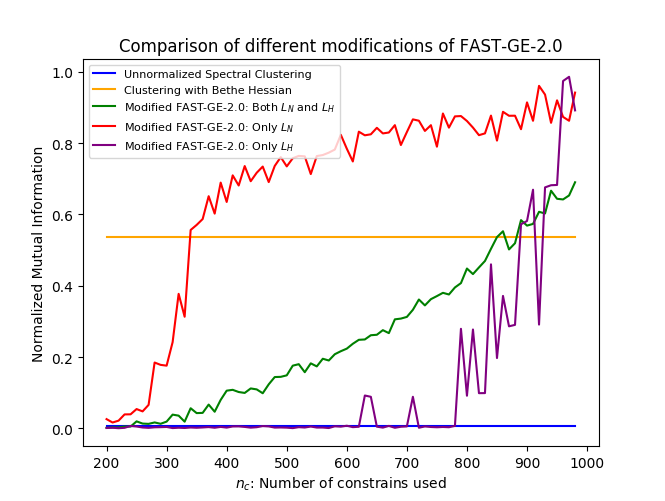
\includegraphics[width=14cm]{figures/CDV1.png}
\end{center}
   \caption[Experimental results for constrained clustering using five different methods]{Experimental results for constrained clustering using five different methods: unnormalized clustering, Bethe Hessian clustering, modified FAST-GE-2.0: both $L_N$ and $L_H$, modified FAST-GE-2.0: only $L_N$, and modified FAST-GE-2.0: only $L_H$. The horizontal axis represents the number of constraints given to each algorithm and the vertical axis represents the normalized mutual information of the set of clusters found by each algorithm and the true labels.}
\label{CDV}
\end{figure}

\subsection*{Discussion}
The result of this experiment shows that none of the modified versions of FAST-GE-2.0 halt.
We can also see that the only one that is able to beat the Bethe Hessian clustering is the modified version of FAST-GE-2.0 where only $L_N$ is substituted by the Bethe Hessian $H_N$, and it does so when about 35\% of the labels are given to the algorithm.
Furthermore, we can also see that after the point where about 40\% of the labels are given to the modified FAST-GE-2.0 algorithm, giving more labels to it does not increase its efficiency much (compared to the interval from 20\% to 40\% of labels).


\section{Experiment 4}
\subsection*{Objective}
Our objective in this final numerical experiment is
\begin{enumerate}[(1)]
   \item to check the efficiency of the modified FAST-GE-2.0: only $L_N$ algorithm for clustering graphs generated by SBM as a function of the difference $c_\text{in} - c_\text{out}$, comparing it to unnormalized clustering and Bethe Hessian clustering; and
   \item to find out how well the modified FAST-GE-2.0 algorithm does when the task is to cluster graphs generated by SBM for more than two clusters (more specifically, for three and five clusters).
\end{enumerate}

\subsection*{Description}
For each $k \in \{ 2, 3, 5 \}$, where $k$ is a parameter of the SBM model, we performed the following numerical experiment: while keeping $c_\text{in} + c_\text{out} = 3$ fixed, for two hundred values of $c_\text{in} - c_\text{out}$ varying equally spaced in the intervals considered in this experiment's figures, we used the stochastic block model to construct ten graphs of size $m = 10000$ for $k$ clusters. Then we used unnormalized spectral clustering and Bethe Hessian clustering to perform clustering, and modified FAST-GE-2.0: only $L_N$ to perform constrained clustering for 25\%, 50\% and 75\% of labels given, respectively.
Finally, we computed the normalized mutual information of each of these sets of clusters and took the average NMI for each algorithm.


\subsection*{Results}
The results from this experiment are shown in Figure~\ref{ACDV1}, Figure~\ref{ACDV2} and Figure~\vref{ACDV3}.

\begin{figure}[h]
\begin{center}
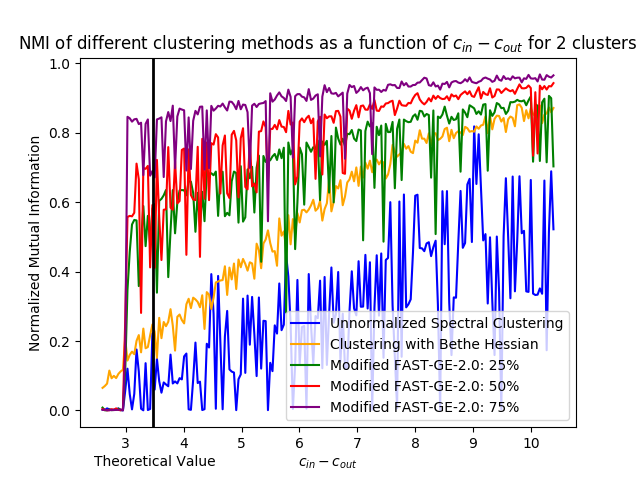
\includegraphics[width=14cm]{figures/ACDV1.png}
\end{center}
   \caption[Experimental results for clustering and constrained clustering as a function of $c_\text{in} - c_\text{out}$ for the number of communities $k=2$]{Experimental results for clustering and constrained clustering as a function of $c_\text{in} - c_\text{out}$ for the number of communities $k=2$. Here we have used two methods for ordinary clustering: unnormalized spectral clustering and Bethe Hessian clustering; and the modified version of FAST-GE-2.0: only $L_N$ for constrained clustering with the amount of labels given to the algorithm being 25\%, 50\% and 75\%. The horizontal axis represents the value of $c_\text{in} - c_\text{out}$ and the vertical axis represents the normalized mutual information of the set of clusters found by each algorithm and the true labels. The black vertical line represents the theoretical limit discussed in Chapter~\ref{bethechapter}.}
\label{ACDV1}
\end{figure}

\begin{figure}[h]
\begin{center}
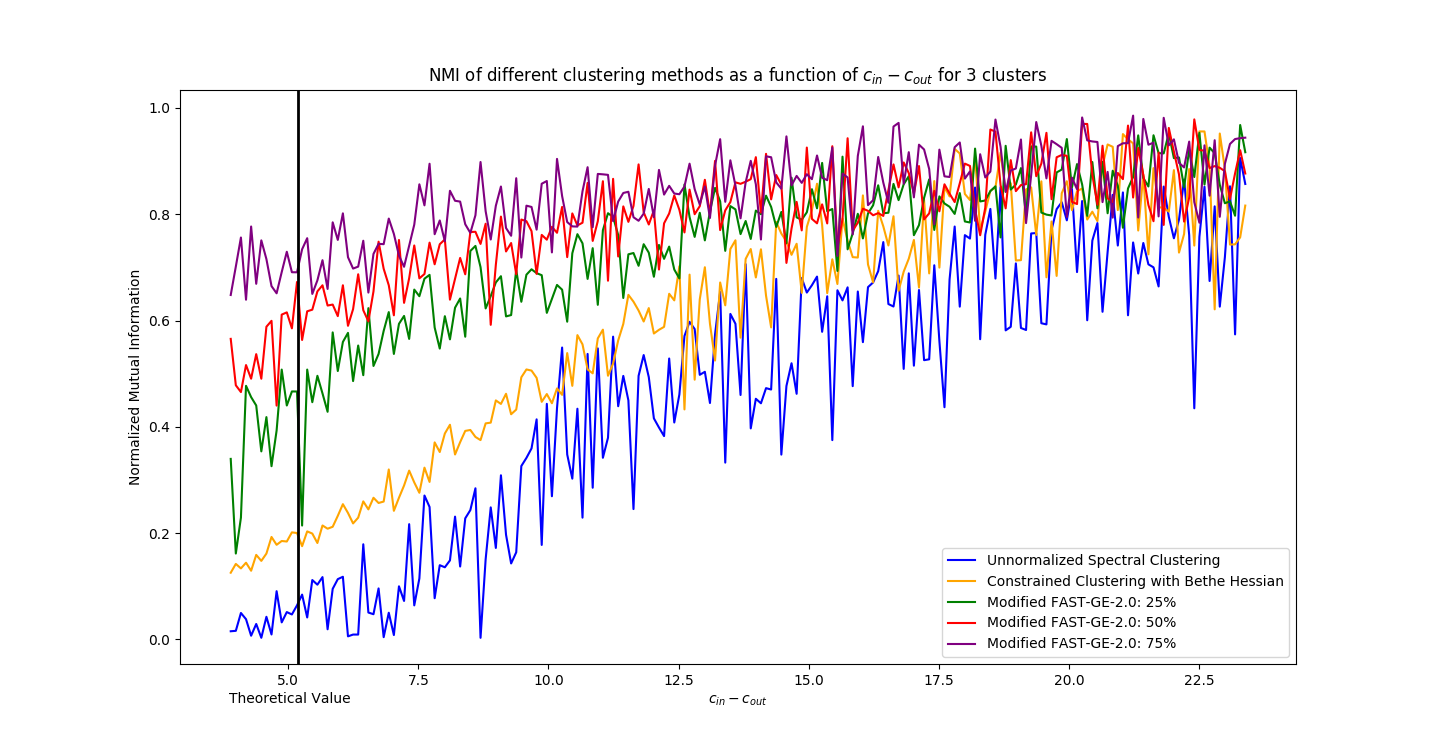
\includegraphics[width=13cm]{figures/ACDV2.png}
\end{center}
   \caption[Experimental results for clustering and constrained clustering as a function of $c_\text{in} - c_\text{out}$ for the number of communities $k=3$]{Experimental results for clustering and constrained clustering as a function of $c_\text{in} - c_\text{out}$ for the number of communities $k=3$. Here we have used two methods for ordinary clustering: unnormalized spectral clustering and Bethe Hessian clustering; and the modified version of FAST-GE-2.0: only $L_N$ for constrained clustering with the amount of labels given to the algorithm being 25\%, 50\% and 75\%. The horizontal axis represents the value of $c_\text{in} - c_\text{out}$ and the vertical axis represents the normalized mutual information of the set of clusters found by each algorithm and the true labels. The black vertical line represents the theoretical limit discussed in Chapter~\ref{bethechapter}.}
\label{ACDV2}
\end{figure}

\begin{figure}[h]
\begin{center}
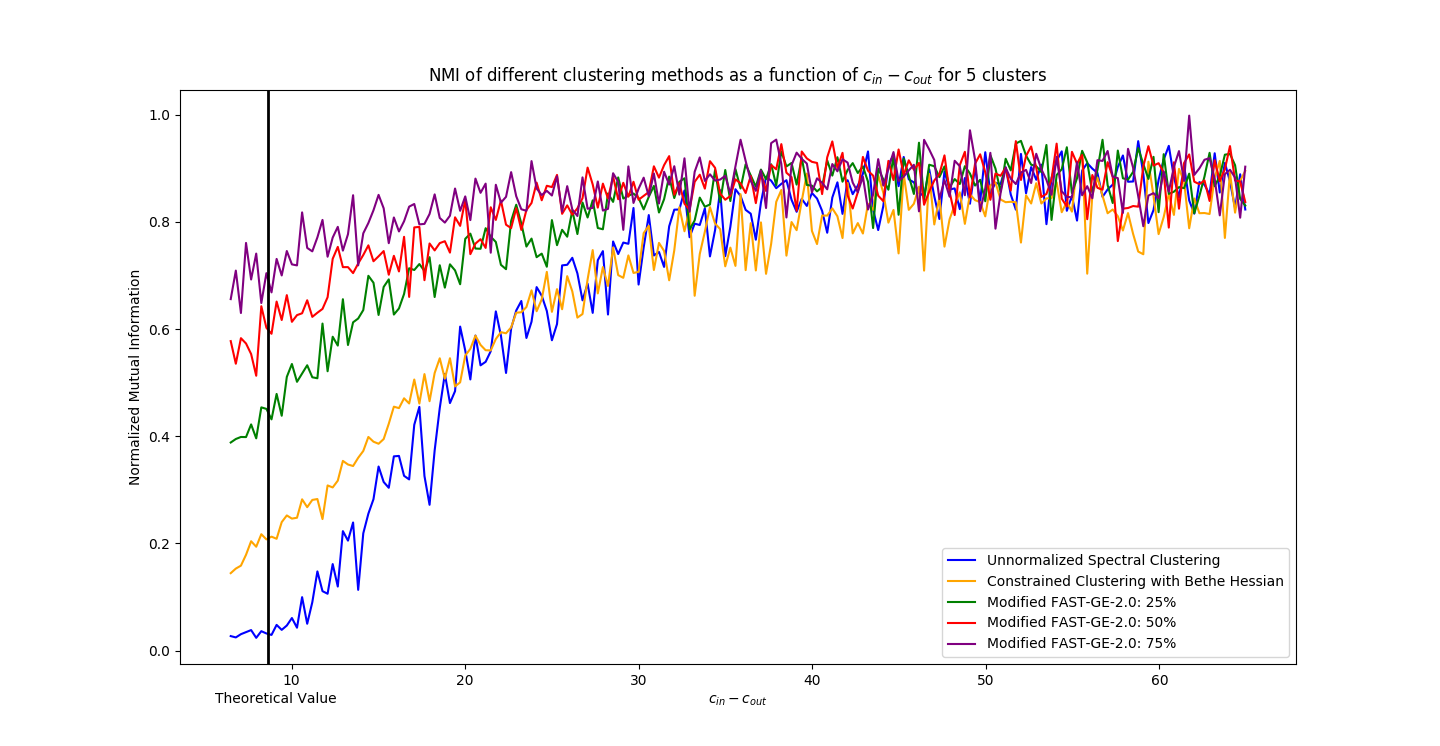
\includegraphics[width=14cm]{figures/ACDV3.png}
\end{center}
   \caption[Experimental results for clustering and constrained clustering as a function of $c_\text{in} - c_\text{out}$ for the number of communities $k=5$]{Experimental results for clustering and constrained clustering as a function of $c_\text{in} - c_\text{out}$ for the number of communities $k=5$. Here we have used two methods for ordinary clustering: unnormalized spectral clustering and Bethe Hessian clustering; and the modified version of FAST-GE-2.0: only $L_N$ for constrained clustering with the amount of labels given to the algorithm being 25\%, 50\% and 75\%. The horizontal axis represents the value of $c_\text{in} - c_\text{out}$ and the vertical axis represents the normalized mutual information of the set of clusters found by each algorithm and the true labels. The black vertical line represents the theoretical limit discussed in Chapter~\ref{bethechapter}.}
   \label{ACDV3}
\end{figure}

\subsection*{Discussion}
The results of this experiment show to us that our proposed method is still better than the Bethe Hessian clustering algorithm and unnormalized spectral clustering algorithm for any value of $c_\text{in} - c_\text{out}$ and for the three values of $k$ we considered in this experiment.
Furthermore, we can see from the experiments the following surprising result: even if just a bit of labels (25\%) are given to our proposed method, it can still get values as high as $0.5$ for the NMI even for values of $c_\text{in} - c_\text{out}$ \textit{smaller} the theoretical value for the limit.
This suggests that the theoretical limit of $c_\text{in} - c_\text{out}$ for graphs generated by the SBM can be considerably lowered if a number of labels, even a small number, is provided together with the graphs.




\chapter{Summary and future work}
In this thesis we have used the standard results from spectral graph theory to derive the well known spectral clustering algorithm. 
After that, we provided a description of the stochastic block model for generating graphs, justified why spectral clustering fails to cluster the graphs generated by it, and introduced a new way of performing clustering that does not suffer from the same problems.
Next we outlined FAST-GE-2.0, a spectral algorithm to perform constrained clustering.
We then explained why FAST-GE-2.0 does not work on graphs generated by SBM and proposed a new algorithm that is able to perform constrained clustering in those graphs.
Finally, we performed numerical experiments that showed the proposed algorithm not only works properly on graphs generated by SBM, but also has surprisingly good performance even when a relatively small amount of data is given to it.

It remains as future work 
\begin{itemize}
   \item to find out why, and give a theoretical explanation of why, is it that modifying only the matrix $L_N$ is better than modifying both the matrices $L_N$ and $L_H$ or only modifyin the matrix $L_H$, and
   \item to test how well do the spectral algorithms we have introduced in this thesis do with graphs generated by a generalized version of the stochastic block model (weighted graph), and
   \item apply the proposed methods to sparse graphs originated from real-world data.
\end{itemize}


\chapter*{Acknowledgements}
\addcontentsline{toc}{chapter}{\numberline{}Acknowledgements}

\newpage

\addcontentsline{toc}{chapter}{\numberline{}References}
\renewcommand{\bibname}{References}

%% 参考文献に jbibtex を使う場合
\bibliographystyle{plain}
\bibliography{report}{}
%% [compile] jbibtex sample; platex sample; platex sample;


\end{document}
